% !TeX program = pdflatex
% !TeX encoding = UTF-8
% !BIB program = biber

\documentclass[a4paper,oneside,11pt,english]{scrartcl}

\usepackage[utf8]{inputenc}
\usepackage[T1]{fontenc}
\usepackage[english]{babel}
\usepackage{graphicx}
\usepackage{amsmath}
\usepackage{amssymb}
\usepackage{booktabs}
\usepackage{hyperref}
\usepackage[margin=2.5cm]{geometry}
\usepackage{caption}
\usepackage{subcaption}
\usepackage{float}
\usepackage{csquotes}
\usepackage{tikz}
\usetikzlibrary{positioning,arrows.meta,shapes,calc,fit,backgrounds}
\usepackage[backend=biber,citestyle=numeric,sortcites=true,maxcitenames=2,style=numeric-comp]{biblatex}

\addbibresource{references.bib}

\hypersetup{
    colorlinks=true,
    linkcolor=blue,
    citecolor=blue,
    urlcolor=blue,
}

\title{%
    Implicit Neural Representations for Image Compression:\\
    An Empirical Study of Batch Size Effects on Training Dynamics
    and Reconstruction Quality
}
\subtitle{Bachelor's Thesis}
\author{Nikita Lutcenko\\[0.3em]
    \small Institute of Machine Learning\\
    \small Johannes Kepler University Linz\\
    \small Upper Austria, Austria\\
    \small \texttt{svetllucenko@gmail.com}\\[0.8em]
    \small \textit{Supervisor:} Gianluca Galletti
}
\date{April 24, 2026}

\begin{document}

\maketitle

% ===================================================================
\begin{abstract}
Implicit neural representations (INRs) store an image as the weights of a
small neural network that maps pixel coordinates to colour, offering a
resolution-independent and differentiable alternative to classical codecs.
For per-image compression, the network is fit to one image at a time, and
the batch size used during this overfitting phase is typically chosen by
convention.  Because every pixel comes from the same spatially correlated
signal, it is not obvious that this choice is harmless, and the present
thesis quantifies what is actually at stake.

We retrain SIREN and COIN on the 24 Kodak images across five batch sizes
(256 pixels up to full-batch), three wall-clock budgets, and three
coarse-to-fine schedules, roughly 1{,}500 training runs in total.  Beyond
PSNR and SSIM, we report a spectral band-wise error obtained from the
Fourier transform of the reconstruction, which localises where quality is
lost between low, middle, and high frequencies.

Batch size turns out to be a first-class design choice in this regime:
across the sweep, average PSNR spans more than 12\,dB.  A simple
coarse-to-fine schedule that starts on a small batch and switches to
full-batch recovers most of the full-batch quality at roughly 56\% of its
training time, which we take as the most practically useful outcome of
the study.

\medskip\noindent
\textit{Code and experiments are available at}
\url{https://github.com/HopeAnAustruanStudent/thesis-inr}.
\end{abstract}

\tableofcontents
\bigskip

% ===================================================================
\section{Introduction}
\label{sec:introduction}

\subsection{Motivation}

Traditional image compression pipelines---JPEG~\cite{wallace1992jpeg},
JPEG\,2000~\cite{taubman2002jpeg2000}, and WebP~\cite{google2010webp}---rely
on hand-crafted transforms (DCT, wavelets) followed by quantization and
entropy coding.  While effective, these methods are limited to a fixed set
of design choices and do not naturally support continuous querying at arbitrary
resolution.

Implicit neural representations (INRs) offer a fundamentally different
alternative: an image is stored as the weights of a small neural network
$f_\theta\colon \mathbb{R}^2 \to \mathbb{R}^3$ that maps normalized pixel
coordinates $(x,y)$ to RGB values.  Since the seminal SIREN
work~\cite{sitzmann2020siren}, numerous extensions have demonstrated
competitive compression ratios while additionally providing resolution
independence and differentiability~\cite{dupont2021coin, dupont2022coinpp,
strumpler2022implicit}.

A key practical question---how does \emph{batch size} during the per-image
overfitting phase affect the quality--speed trade-off?---remains underexplored.
Training on all pixels at once (full-batch) guarantees an unbiased gradient at
each step but is memory-intensive; smaller mini-batches introduce stochasticity
that may help or hinder convergence.  In standard deep learning, mini-batch
stochasticity is often beneficial for generalization~\cite{keskar2017largebatch}.
However, the INR setting---where the network overfits to a \emph{single}
signal with spatially correlated pixels---differs fundamentally from the
i.i.d.\ sampling assumption, and batch size effects in this regime are less
understood.

\begin{figure}[H]
\centering
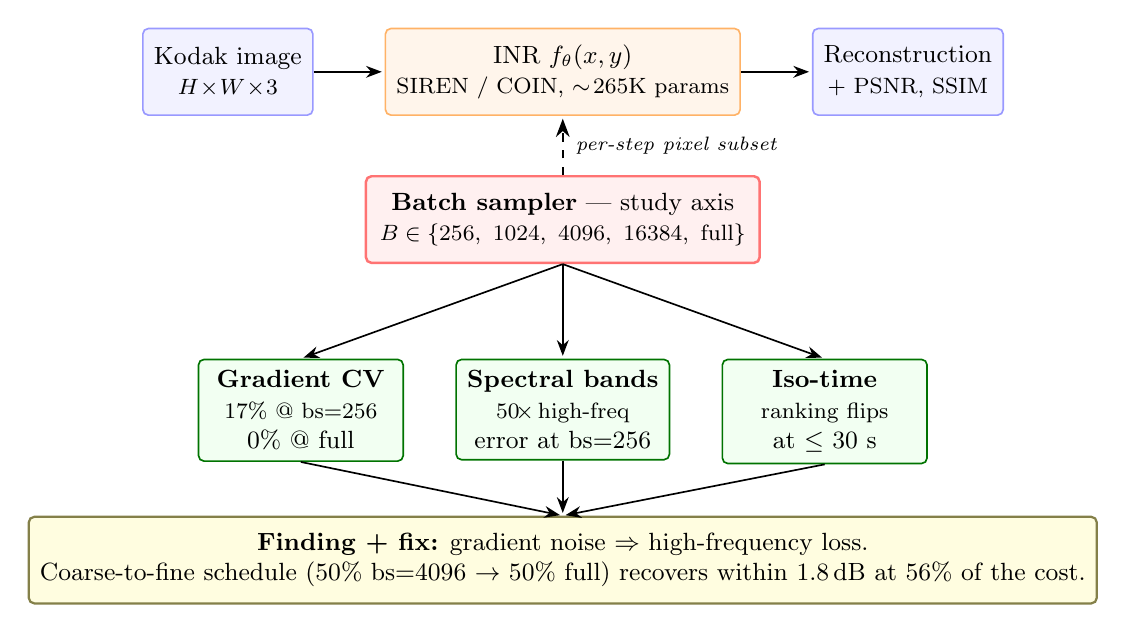
\begin{tikzpicture}[
    font=\small,
    >=Stealth,
    every node/.style={align=center},
    box/.style={draw, rounded corners=2pt, minimum height=1.1cm, inner sep=4pt, line width=0.6pt},
    data/.style={box, fill=blue!5, draw=blue!40},
    model/.style={box, fill=orange!8, draw=orange!60, minimum width=3.2cm},
    study/.style={box, fill=red!6, draw=red!55, line width=0.9pt},
    analysis/.style={box, fill=green!5, draw=green!45!black, minimum width=2.6cm},
    arrow/.style={->, line width=0.6pt, shorten >=1pt}
]
% Top row: pipeline
\node[data] (img) {Kodak image\\ \footnotesize $H\!\times\!W\!\times\!3$};
\node[model, right=0.9cm of img] (inr) {INR $f_\theta(x,y)$\\ \footnotesize SIREN / COIN, $\sim\!265$K params};
\node[data, right=0.9cm of inr] (recon) {Reconstruction\\ \footnotesize + PSNR, SSIM};

\draw[arrow] (img) -- (inr);
\draw[arrow] (inr) -- (recon);

% Batch sampler feeding into the INR
\node[study, below=0.75cm of inr, minimum width=5cm] (sampler) {%
    \textbf{Batch sampler} --- study axis\\
    \footnotesize $B \in \{256,\ 1024,\ 4096,\ 16384,\ \text{full}\}$};
\draw[arrow, dashed, line width=0.8pt] (sampler.north) -- (inr.south)
    node[midway, right=1pt, font=\scriptsize\itshape] {per-step pixel subset};

% Analysis branches
\node[analysis, below left=1.2cm and -0.5cm of sampler] (ga) {%
    \textbf{Gradient CV}\\ \footnotesize 17\% @ bs=256\\ 0\% @ full};
\node[analysis, below=1.2cm of sampler] (sp) {%
    \textbf{Spectral bands}\\ \footnotesize $50\!\times\!$ high-freq\\ error at bs=256};
\node[analysis, below right=1.2cm and -0.5cm of sampler] (it) {%
    \textbf{Iso-time}\\ \footnotesize ranking flips\\ at $\le$ 30 s};

\draw[arrow] (sampler.south) -- (ga.north);
\draw[arrow] (sampler.south) -- (sp.north);
\draw[arrow] (sampler.south) -- (it.north);

% Outcome
\node[box, fill=yellow!12, draw=yellow!45!black, below=0.7cm of sp, minimum width=8cm, line width=0.8pt] (out) {%
    \textbf{Finding + fix:} gradient noise $\Rightarrow$ high-frequency loss.\\
    Coarse-to-fine schedule (50\% bs=4096 $\rightarrow$ 50\% full) recovers within 1.8\,dB at 56\% of the cost.};

\draw[arrow] (ga.south) -- (out.north);
\draw[arrow] (sp.south) -- (out.north);
\draw[arrow] (it.south) -- (out.north);
\end{tikzpicture}
\caption{Overview of the study.  An INR (SIREN or COIN) is trained to overfit
a single Kodak image.  The only axis we vary is the batch of pixels used per
gradient step; we then measure gradient coefficient of variation, spectral
band-wise error, and iso-time reconstruction quality, and use those
measurements to motivate a coarse-to-fine training schedule.}
\label{fig:overview}
\end{figure}

\subsection{Objectives}

The ambition of this research is three-fold:

\begin{enumerate}
    \item To systematically measure how batch size affects reconstruction
          quality, spectral fidelity, and training efficiency in INR-based
          image compression.
    \item To determine whether this effect is architecture-dependent by
          comparing SIREN (sinusoidal activations) and COIN (ReLU with
          positional encoding).
    \item To identify the underlying mechanism behind the batch size effect
          through gradient variance analysis, and to propose practical
          strategies (adaptive scheduling) to mitigate the quality--speed
          trade-off.
\end{enumerate}

Formally, INR-based image compression solves the following optimization for each
image $\mathcal{I}$:
\begin{equation}
    \min_\theta \;\frac{1}{|\mathcal{B}|} \sum_{(x_i,y_i) \in \mathcal{B}}
    \bigl\| f_\theta(x_i) - y_i \bigr\|^2,
    \label{eq:objective}
\end{equation}
where $f_\theta$ is a coordinate-based MLP, $(x_i, y_i)$ are pixel coordinates
and RGB values, and $\mathcal{B}$ is the batch of pixels sampled at each step.
When $|\mathcal{B}| = H \times W$ (full-batch), the gradient is exact; when
$|\mathcal{B}| \ll H \times W$, the gradient is a stochastic approximation
over a spatially-correlated signal.  Fig.~\ref{fig:overview} summarizes the
study at a glance: the batch size is the only axis we vary, and the
gradient-variance, spectral-band, and iso-time measurements drive the
coarse-to-fine schedule that closes the paper.

\subsection{Thesis Structure}

The remainder of this thesis is organized as follows:

\begin{itemize}
    \item \textbf{Section~\ref{sec:background}: Background and Related Work} ---
          provides an overview of INR architectures, spectral bias, and batch
          size theory in deep learning.
    \item \textbf{Section~\ref{sec:methodology}: Methodology} --- presents the
          model architectures, sampling strategies, training procedures, and
          evaluation metrics.
    \item \textbf{Section~\ref{sec:experiments}: Experiments and Results} ---
          describes the experimental setup, presents quantitative results
          across eleven experiments, and discusses findings.
    \item \textbf{Section~\ref{sec:conclusion}: Conclusion and Future Work} ---
          summarizes contributions and outlines directions for future research.
\end{itemize}


% ===================================================================
\section{Notation}
\label{sec:notation}

Throughout this thesis, specific notation is used consistently.
The image is denoted $\mathcal{I} \in [0,1]^{H \times W \times 3}$ with height
$H$ and width $W$.  Pixel coordinates are normalized to $[-1,1]^2$ and denoted
$(x, y)$.  The coordinate-based MLP is $f_\theta\colon \mathbb{R}^2 \to
\mathbb{R}^3$, parameterized by weights $\theta$.  The batch of sampled pixels
at step $t$ is $\mathcal{B}_t$, with $|\mathcal{B}_t| = B$ (the batch size).
The full pixel set is $\mathcal{P} = \{(x_i, y_i)\}_{i=1}^{HW}$.  The
stochastic gradient at step $t$ is:
\begin{equation}
    \hat{g}_t = \frac{1}{B} \sum_{(x,y) \in \mathcal{B}_t}
    \nabla_\theta \bigl\| f_\theta(x, y) - \mathcal{I}(x, y) \bigr\|^2
\end{equation}
and the full gradient is $g_t = \hat{g}_t \big|_{B = HW}$.  The gradient
variance is $\text{Var}[\hat{g}_t] = \mathbb{E}[\|\hat{g}_t - g_t\|^2]$,
which decreases with $B$.

Code references use \texttt{typewriter font}, e.g., \texttt{SIREN},
\texttt{random\_pixels(n)}.  Metrics are abbreviated as PSNR (Peak
Signal-to-Noise Ratio, in dB), SSIM~\cite{wang2004ssim} (Structural
Similarity Index, unitless in $[0,1]$), and
LPIPS~\cite{zhang2018lpips} (Learned Perceptual Image Patch Similarity,
lower is better).

% ===================================================================
\section{Background and Related Work}
\label{sec:background}

\subsection{Implicit Neural Representations}

An implicit neural representation (INR) encodes a signal (image, audio, 3D
shape) as a continuous function parameterized by a neural network.  For images,
the network $f_\theta(x,y) \to (r,g,b)$ maps 2D coordinates to color values.
The ``compression'' comes from storing the network weights (typically
$\sim$250k parameters $\approx$ 1\,MB) instead of the raw pixel grid.

Formally, the encoding process solves:
\begin{equation}
    \theta^* = \arg\min_\theta \frac{1}{HW} \sum_{i=1}^{HW}
    \bigl\| f_\theta(x_i, y_i) - (r_i, g_i, b_i) \bigr\|^2
\end{equation}
where $(x_i, y_i) \in [-1, 1]^2$ are normalized pixel coordinates and
$(r_i, g_i, b_i) \in [0, 1]^3$ are the corresponding RGB values.  Once
$\theta^*$ is found, the image can be decoded at any resolution by evaluating
$f_{\theta^*}$ at arbitrary coordinates --- this is the key advantage of INRs
over discrete pixel representations.

The key challenge is \emph{spectral bias}: standard neural networks with ReLU
activations learn low-frequency functions first and struggle with
high-frequency details.  This phenomenon was first identified and named by
Rahaman et~al.~\cite{rahaman2019spectral}, who showed that the convergence
rate of neural networks is frequency-dependent, with low-frequency components
being learned orders of magnitude faster than high-frequency ones.  Tancik
et al.~\cite{tancik2020fourier} later demonstrated that this bias can be
overcome in coordinate-based networks by mapping inputs through Fourier
features.  Two main architectural solutions have been proposed: periodic
activations (SIREN) and positional encoding (Fourier features).

It is important to distinguish \emph{network spectral bias}---an inherent
property of network architecture and activation functions---from what we term
\emph{sampling-induced spectral degradation}, where the choice of training
samples (batch size and spatial distribution) affects which frequency
components are effectively learned.  This distinction is central to the
present study: even when using architectures designed to overcome network
spectral bias (SIREN, Fourier features), suboptimal sampling may introduce
a separate, optimization-level frequency bias.

\subsection{SIREN}
\label{sec:siren}

Sitzmann et al.~\cite{sitzmann2020siren} introduced SIREN (Sinusoidal
Representation Networks), replacing the standard ReLU activation with a
periodic sinusoidal function:
\begin{equation}
    \phi_l(\mathbf{x}) = \sin\bigl(\omega_0 \cdot (\mathbf{W}_l \mathbf{x}
    + \mathbf{b}_l)\bigr)
\end{equation}
where $\omega_0$ is a hyperparameter controlling the frequency capacity of
each layer.  The multiplication by $\omega_0$ before applying $\sin(\cdot)$
allows the network to represent signals with frequency content up to
$\omega_0 / 2$ per layer.

A single SIREN layer performs:
\begin{equation}
    \mathbf{h}_l = \sin\bigl(\omega_0 \cdot (\mathbf{W}_l \mathbf{h}_{l-1}
    + \mathbf{b}_l)\bigr), \quad l = 1, \ldots, L
\end{equation}
with the final output layer using a sigmoid activation to map to $[0, 1]$:
$\mathbf{o} = \sigma(\mathbf{W}_{L+1} \mathbf{h}_L + \mathbf{b}_{L+1})$.

\paragraph{Weight Initialization.}
Standard random initialization (e.g., Xavier~\cite{glorot2010xavier},
Kaiming~\cite{he2015delving}) does not work for SIREN because the
sinusoidal activation requires specific input statistics to avoid
saturation or underutilization.  Sitzmann et al.\ derive a
principled initialization scheme that preserves the distribution of
activations across layers:
\begin{itemize}
    \item \textbf{First layer}: $\mathbf{W}_1 \sim
          \mathcal{U}(-1/n, \; 1/n)$ where $n$ is the fan-in (number of input
          features).  This ensures the input to $\sin(\cdot)$ spans $[-1, 1]$
          when coordinates are in $[-1, 1]$.
    \item \textbf{Hidden layers}: $\mathbf{W}_l \sim
          \mathcal{U}\bigl(-\sqrt{6/n}\,/\,\omega_0,\;
          \sqrt{6/n}\,/\,\omega_0\bigr)$.  The $\sqrt{6/n}$ factor comes
          from variance preservation (analogous to Xavier initialization),
          divided by $\omega_0$ to account for the frequency scaling.
\end{itemize}

\paragraph{Why $\omega_0 = 30$?}
Higher $\omega_0$ increases the frequency capacity but makes training less
stable.  Sitzmann et al.\ empirically found $\omega_0 = 30$ to work well
for natural image fitting.  This value allows the network to represent
frequencies up to approximately 15 cycles per unit coordinate, which is
sufficient for most natural images at Kodak resolution.

\subsection{COIN and Positional Encoding}
\label{sec:coin}

COIN~\cite{dupont2021coin} takes a fundamentally different approach to
overcoming spectral bias.  Instead of modifying the activation function,
it modifies the \emph{input} using a Fourier positional encoding:
\begin{equation}
    \gamma(\mathbf{p}) = \bigl[\sin(2^0 \pi \mathbf{p}), \;
    \cos(2^0 \pi \mathbf{p}), \; \ldots, \;
    \sin(2^{L-1} \pi \mathbf{p}), \;
    \cos(2^{L-1} \pi \mathbf{p})\bigr]
\end{equation}
where $\mathbf{p} \in \mathbb{R}^2$ is the input coordinate and $L = 10$
is the number of frequency octaves.  This maps each 2D coordinate to a
40-dimensional feature vector ($2 \times 10 \times 2 = 40$), explicitly
providing the network with sinusoidal features at frequencies
$\pi, 2\pi, \ldots, 512\pi$.

The key difference from SIREN is where frequency information enters the
network:
\begin{itemize}
    \item \textbf{SIREN}: frequencies are generated by the \emph{activation
          function} at every layer.  The network learns which frequencies to
          combine.
    \item \textbf{COIN}: frequencies are provided at the \emph{input} level
          and are fixed.  The ReLU network learns to combine these fixed
          frequency features.
\end{itemize}

This distinction is central to our thesis: if batch size affects these
architectures differently, it reveals how gradient information interacts
with the frequency-encoding mechanism.

COIN was originally designed for a meta-learning pipeline (MAML-based
initialization amortized across images)~\cite{dupont2022coinpp}.  In this
work, we evaluate the architectural component in the single-image
overfitting setting to isolate the effect of activation function choice.
The COIN results should therefore not be compared directly to published
COIN numbers, which benefit from meta-learned initialization.

\subsection{Other INR Architectures}

Beyond SIREN and COIN, several architectures have been proposed.
WIRE~\cite{saragadam2023wire} uses complex Gabor wavelets as activations,
achieving competitive results on image fitting with improved spatial
localization compared to SIREN's global sinusoidal basis.
Gaussian activation networks~\cite{ramasinghe2022beyond} and multiplicative
filter networks~\cite{fathony2021multiplicative} offer alternative approaches
to overcoming spectral bias.  NeRF~\cite{mildenhall2020nerf} extended
coordinate-based representations to 3D scenes, demonstrating the generality
of the INR paradigm beyond 2D images.

\subsection{INR Compression and Rate-Distortion}

Weight quantization and entropy coding are essential for competitive INR
compression.  Str\"umpler et al.~\cite{strumpler2022implicit} proposed
entropy-constrained training where quantization is incorporated into the
training loop, achieving bitrates competitive with learned compression
methods.  COIN++~\cite{dupont2022coinpp} introduces modulation-based
meta-learning to amortize the per-image fitting cost across a dataset.
MINER~\cite{saragadam2022miner} proposes a multi-scale tree structure where
different spatial regions are represented at different resolutions, effectively
implementing a hierarchical spatial sampling strategy.

In the broader context of learned image compression, autoencoder-based
methods~\cite{balle2018variational} currently achieve state-of-the-art
rate-distortion performance, significantly outperforming both traditional
codecs and current INR methods.  However, INR compression offers unique
properties (resolution independence, differentiability, compact functional
form) that motivate continued research into training efficiency.

The present study is orthogonal to weight compression: we investigate
\emph{how to train the network effectively}, not how to compress its weights.
Improvements in training efficiency (such as optimal batch size selection or
adaptive scheduling) compose with any downstream weight compression technique.

\subsection{Batch Size in Neural Network Training}

The interplay between batch size, learning rate, and generalization has been
studied extensively in the supervised learning
setting~\cite{keskar2017largebatch, smith2018dont}.  The linear scaling
rule~\cite{goyal2017accurate} prescribes adjusting the learning rate
proportionally to batch size.  However, these results assume i.i.d.\
mini-batch sampling from a large dataset.  The INR setting---where the
network overfits to a single signal with spatially correlated pixels---differs
fundamentally.  To our knowledge, no prior work has systematically studied how
batch size interacts with architecture choice and frequency-domain
reconstruction quality in INR-based compression.


% ===================================================================
\section{Methodology}
\label{sec:methodology}

\subsection{Data Collection}

We use the Kodak PhotoCD dataset~\cite{kodak}, a standard benchmark for image compression
research containing 24 images at $768 \times 512$ or $512 \times 768$
resolution.  Each image contains $H \times W \times 3 = 1{,}179{,}648$ bytes
uncompressed.  The dataset is downloaded programmatically via a provided
script (\texttt{data/download\_kodak.py}) from the public Kodak mirror and
stored as uncompressed PNG files.  All pixel values are normalized to $[0,1]$
by dividing by 255.  No augmentation or other preprocessing is applied.

The choice of Kodak is motivated by its widespread use in the compression
literature, enabling direct comparison with published results.  However, it
represents a limited evaluation at a single resolution (see
Section~\ref{sec:limitations}).

\subsection{Model Architectures}
\label{sec:architectures}

Both architectures are implemented in PyTorch and follow a modular design
that separates the model definition from the training loop and evaluation
pipeline.  Table~\ref{tab:architecture} summarizes the key architectural
differences.

\begin{table}[H]
\centering
\caption{Comparison of the two architectures used in this study.}
\label{tab:architecture}
\begin{tabular}{lcc}
\toprule
Property & SIREN & COIN \\
\midrule
Activation & $\sin(\omega_0 \cdot x)$ & ReLU \\
Input processing & Direct coordinates & Positional encoding ($L=10$) \\
Input dimension & 2 & 40 \\
Hidden layers & 5 $\times$ 256 & 5 $\times$ 256 \\
Output activation & Sigmoid & Sigmoid \\
Initialization & SIREN-specific & Kaiming uniform \\
Parameters & 264{,}707 & 274{,}435 \\
Size (float32) & 1.01\,MB & 1.02\,MB \\
Size (float16) & 517\,KB & 521\,KB \\
\bottomrule
\end{tabular}
\end{table}

\subsubsection{SIREN Implementation}

The SIREN model is implemented in \texttt{models/siren.py} as two classes:
\texttt{SineLayer} (a single sinusoidal layer) and \texttt{SIREN} (the
full network).  The architecture is:

\begin{equation}
    (x, y) \xrightarrow{\text{SineLayer}(2, 256)}
    \mathbf{h}_1 \xrightarrow{\text{SineLayer}(256, 256)} \cdots
    \xrightarrow{\text{SineLayer}(256, 256)}
    \mathbf{h}_5 \xrightarrow{\text{Linear}(256, 3)}
    \xrightarrow{\sigma(\cdot)} (r, g, b)
\end{equation}

The total parameter count of 264{,}707 breaks down as: first layer
$2 \times 256 + 256 = 768$; four hidden layers $4 \times (256 \times 256 +
256) = 266{,}240$; output layer $256 \times 3 + 3 = 771$.  This yields a
compression ratio of $\sim$1.13$\times$ at \texttt{float32} and
$\sim$2.26$\times$ at \texttt{float16} for a Kodak image.

\subsubsection{COIN Implementation}

The COIN model is implemented in \texttt{models/coin.py} as two classes:
\texttt{PositionalEncoding} (the Fourier feature mapping) and \texttt{COIN}
(the full network).  The positional encoding expands each 2D coordinate to
40 features:
\begin{equation}
    \gamma(x, y) = [\sin(\pi x), \cos(\pi x), \sin(2\pi x),
    \cos(2\pi x), \ldots, \sin(512\pi x), \cos(512\pi x),
    \text{same for } y]
\end{equation}
These 40 features are then processed by a standard ReLU MLP with Kaiming
initialization.  The total parameter count is 274{,}435, broken down as:
first hidden layer $40 \times 256 + 256 = 10{,}496$; four hidden layers
$4 \times (256 \times 256 + 256) = 263{,}168$; output layer $256 \times 3 + 3 =
771$.  COIN is slightly larger than SIREN (by $\sim$9{,}728 parameters, the
first-layer overhead from the 40-dimensional Fourier feature input).

\subsection{Batch Sampling Strategies}
\label{sec:sampling}

The batch sampling strategy is the central variable of this study.  We
investigate two sampling modes at five batch sizes, implemented in
\texttt{training/sampling.py}:

\begin{enumerate}
    \item \textbf{Full image} (\texttt{full\_image}): all $H \times W$ pixels
          are used at every step (deterministic gradient,
          $|\mathcal{B}| = 393{,}216$ for Kodak).  The gradient is exact:
          $\nabla_\theta \mathcal{L} = \frac{1}{HW} \sum_{i=1}^{HW}
          \nabla_\theta \ell_i$.
    \item \textbf{Random pixels} (\texttt{random\_pixels(n)}): $n$ pixels
          sampled uniformly at random without replacement per step
          (stochastic gradient).  A different subset is drawn at every step.
\end{enumerate}

The batch sizes swept are: 256, 1{,}024, 4{,}096, 16{,}384, and ``full.''
This spans three orders of magnitude, from 0.07\% to 100\% of pixels per
step.  Table~\ref{tab:batch_sizes} shows the spatial coverage of each batch
size.

\begin{table}[H]
\centering
\caption{Batch size configurations and their spatial coverage for a
$768 \times 512$ Kodak image.}
\label{tab:batch_sizes}
\begin{tabular}{lccc}
\toprule
Batch Size & Pixels/Step & \% of Image & Pixels in 2000 Steps \\
\midrule
256      & 256      & 0.07\% & 512{,}000 \\
1{,}024  & 1{,}024  & 0.26\% & 2{,}048{,}000 \\
4{,}096  & 4{,}096  & 1.04\% & 8{,}192{,}000 \\
16{,}384 & 16{,}384 & 4.17\% & 32{,}768{,}000 \\
Full     & 393{,}216 & 100\% & 786{,}432{,}000 \\
\bottomrule
\end{tabular}
\end{table}

The coordinate grid is constructed using \texttt{numpy.linspace} to map
pixel indices to $[-1, 1]$ coordinates.  For random sampling, indices are
drawn using \texttt{numpy.random.choice} without replacement (or with
replacement when $n > HW$, which does not occur in our experiments).

\subsection{Training Procedure}

\subsubsection{Hyperparameters}

All models are trained with the Adam optimizer~\cite{kingma2015adam}
($\text{lr} = 10^{-4}$, $\beta_1 = 0.9$, $\beta_2 = 0.999$) and MSE loss.
The default training budget is 2{,}000 steps.  For iso-time experiments,
training continues until a wall-clock time budget is exhausted (30, 60, or
120 seconds).

\subsubsection{Adaptive Batch-Size Schedule}

Motivated by the observation that low frequencies converge first (spectral
bias), we propose a coarse-to-fine training schedule: the first phase uses
small batches (fast, learns global structure) and the second phase switches
to large batches (slower, refines high-frequency detail).  Three schedules
are tested:
\begin{itemize}
    \item \textbf{A}: 30\% of steps at \texttt{bs=1024}, then 70\% at full.
    \item \textbf{B}: 50\% at \texttt{bs=4096}, then 50\% at full.
    \item \textbf{C}: 20\% at \texttt{bs=256}, 30\% at \texttt{bs=4096},
          50\% at full.
\end{itemize}

\subsubsection{Seeding and Reproducibility}

To verify statistical robustness, we repeat the SIREN sweep with 3 different
random seeds on 6 images and decompose the total PSNR variance into
inter-image and inter-seed components.

\subsection{Evaluation Metrics}

\paragraph{PSNR.}
Peak Signal-to-Noise Ratio measures pixel-level fidelity:
$\text{PSNR} = 10 \cdot \log_{10}(1/\text{MSE})$.

\paragraph{SSIM.}
Structural Similarity Index~\cite{wang2004ssim} captures perceptual similarity
via luminance, contrast, and structural comparisons.

\paragraph{Spectral Error.}
We work in the frequency domain to localize \emph{where} reconstruction
errors live along the spatial-frequency axis.  Let $\mathcal{I},
\hat{\mathcal{I}} \in [0,1]^{H \times W}$ be the luminance channel
($Y = 0.299\,R + 0.587\,G + 0.114\,B$) of the reference and reconstructed
images.  For each, we compute the centered 2D FFT magnitude spectrum and
take its logarithm:
\begin{equation}
    S(u,v) = \log\bigl(1 + \bigl|\mathcal{F}\{\mathcal{I}\}(u,v)\bigr|\bigr),
    \qquad \hat{S}(u,v) = \log\bigl(1 + \bigl|\mathcal{F}\{\hat{\mathcal{I}}\}(u,v)\bigr|\bigr).
    \label{eq:fft_magnitude}
\end{equation}
To reduce the 2D spectrum to a 1D signature, we compute the radially-averaged
power spectrum $P(r) = \mathbb{E}_{\|(u,v) - c\| = r}[\,S(u,v)\,]$, where $c$ is
the spectrum center and $r$ is the radial frequency bin in pixels.  The
analogous quantity $\hat{P}(r)$ is defined for the reconstruction.  The
\emph{band-wise spectral error} partitions $r \in [0, \min(H,W)/2]$ into three
equal-width radial bands and reports the mean squared deviation in each:
\begin{equation}
    E_b = \frac{1}{|\mathcal{R}_b|}\sum_{r \in \mathcal{R}_b}
          \bigl(P(r) - \hat{P}(r)\bigr)^2,
    \qquad b \in \{\text{low}, \text{mid}, \text{high}\}.
    \label{eq:spectral_error}
\end{equation}
$E_{\text{low}}$ captures loss of global structure (large-scale colour and
shape), $E_{\text{mid}}$ captures mid-scale content, and $E_{\text{high}}$
captures sharp edges and fine textures.  Because natural-image spectra decay
roughly as $1/r^\alpha$, the raw magnitudes differ by orders of magnitude
across bands; the logarithm in Eq.~\ref{eq:fft_magnitude} ensures that all
three bands contribute informatively to $E_b$.

\paragraph{Gradient Variance.}
To understand the \emph{mechanism} behind batch size effects, we measure the
coefficient of variation (CV = std/mean) of gradient norms across 30
independent mini-batch samples at fixed model states.

\subsection{Hardware and Compute}

All experiments are run on an NVIDIA GeForce RTX 5060 Ti GPU (16\,GB VRAM)
with CUDA 12.8 and PyTorch 2.10.  The full experimental campaign comprises
approximately 1{,}500 training runs with a total GPU time of $\sim$20 hours.


% ===================================================================
\section{Experiments and Results}
\label{sec:experiments}

\subsection{Experimental Setup}

For each of the 24 Kodak images and each batch size in $\{256, 1024, 4096,
16384, \text{full}\}$, we train a SIREN from scratch, yielding $24 \times 5 = 120$
training runs.  The same sweep is repeated with COIN (120 runs).  Extended
experiments (iso-time, adaptive, gradient variance, LR scaling, difficulty
analysis, VRAM profiling, JPEG comparison, multi-seed) add $\sim$1{,}260
additional runs.

\subsection{SIREN Batch-Size Sweep}

\begin{table}[H]
\centering
\caption{Average PSNR, SSIM, training time, and spectral error across all 24
Kodak images at 2{,}000 fixed steps (mean $\pm$ std).
Note: this comparison is confounded by differing data volumes per step;
the iso-time comparison in Table~\ref{tab:iso_time} provides a fairer
assessment.}
\label{tab:main_results}
\begin{tabular}{lccccc}
\toprule
Batch Size & PSNR (dB) $\uparrow$ & SSIM $\uparrow$ & Time (s) & Spec.\ Low & Spec.\ High \\
\midrule
256    & $21.72 \pm 2.34$ & $0.525 \pm 0.134$ & $26.3$  & $0.3568$ & $4.420$ \\
1024   & $23.69 \pm 2.52$ & $0.622 \pm 0.125$ & $26.3$  & $0.2191$ & $3.974$ \\
4096   & $25.75 \pm 2.72$ & $0.713 \pm 0.101$ & $25.7$  & $0.0344$ & $2.411$ \\
16384  & $28.56 \pm 2.96$ & $0.810 \pm 0.068$ & $30.6$  & $0.0024$ & $0.891$ \\
Full   & $34.19 \pm 2.82$ & $0.920 \pm 0.026$ & $231.9$ & $0.0003$ & $0.087$ \\
\bottomrule
\end{tabular}
\end{table}

PSNR increases monotonically with batch size, spanning +12.5\,dB from
\texttt{bs=256} to full-batch.  High-frequency spectral error drops
50$\times$, confirming that mini-batching disproportionately degrades
high-frequency content.  Mini-batch sizes 256--4096 have nearly identical
wall-clock time ($\sim$26\,s); the overhead is in the per-step
forward/backward pass, not data loading.

\begin{figure}[H]
    \centering
    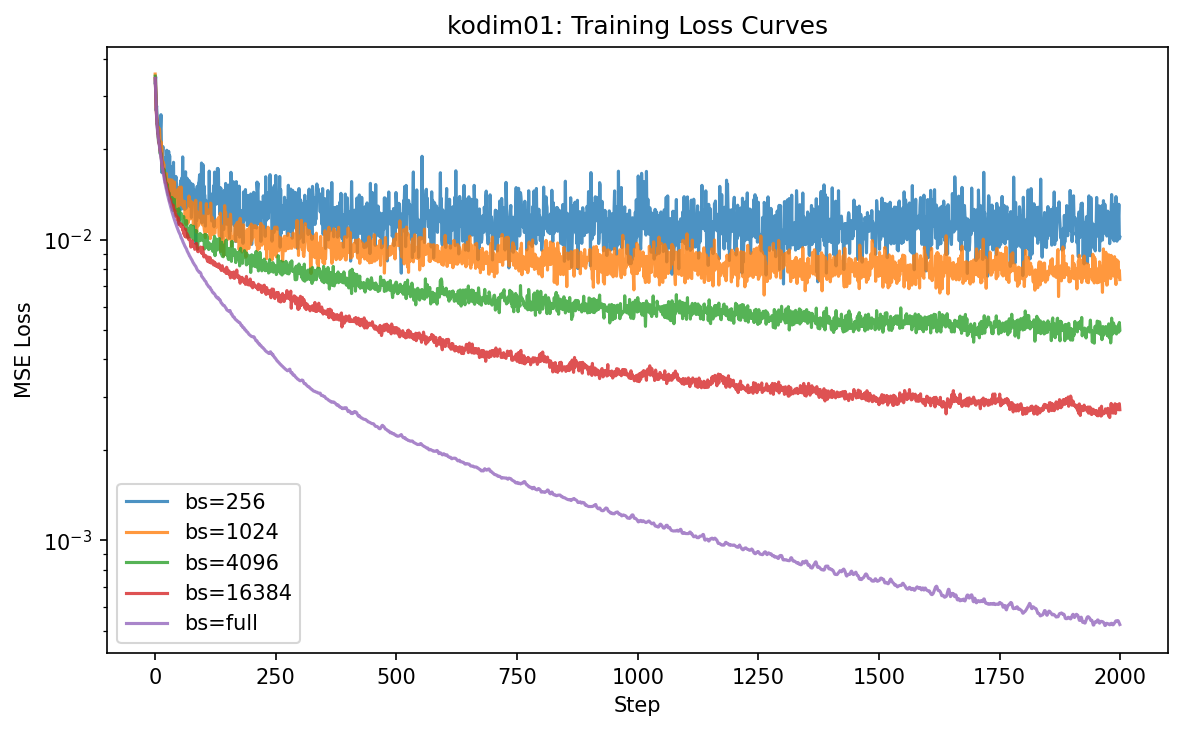
\includegraphics[width=\textwidth]{figures/loss_curves_kodim01.png}
    \caption{Training loss curves for different batch sizes on kodim01.
    Smaller batches converge to higher loss plateaus.}
    \label{fig:loss_curves}
\end{figure}

\begin{figure}[H]
    \centering
    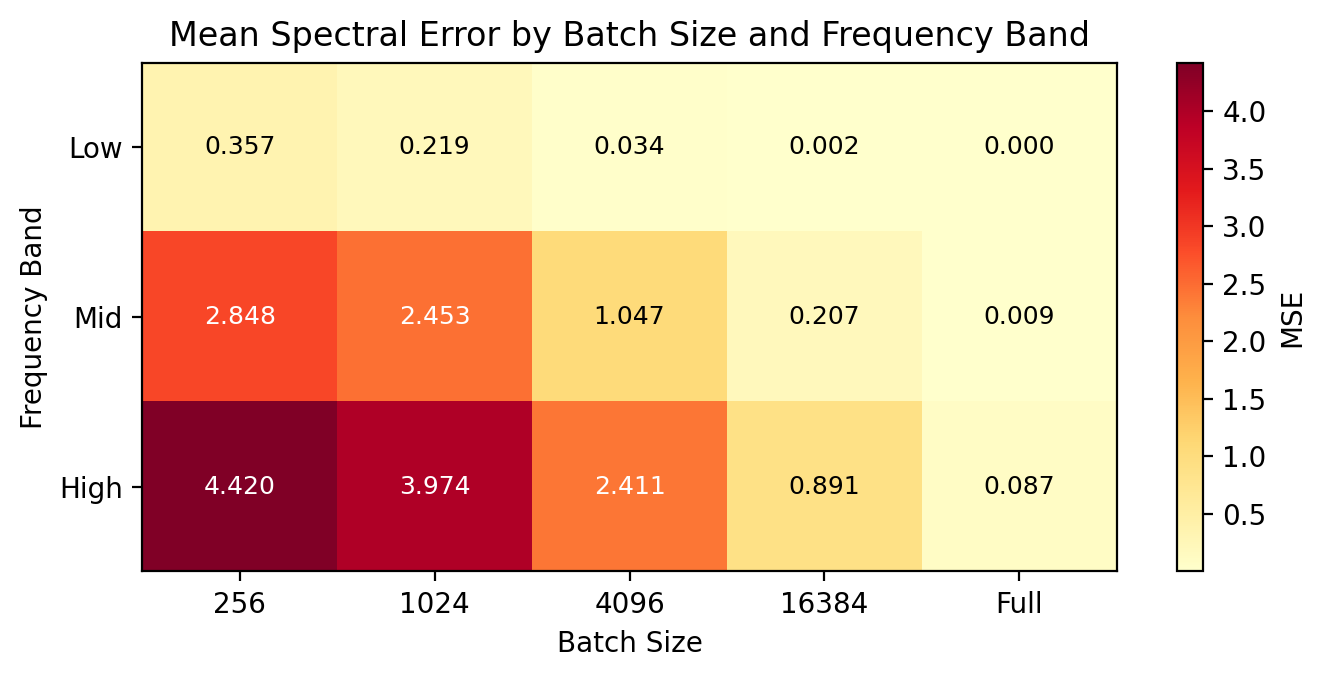
\includegraphics[width=\textwidth]{figures/spectral_heatmap.png}
    \caption{Mean spectral error by batch size and frequency band. Smaller
    batch sizes disproportionately lose high-frequency content.}
    \label{fig:spectral_heatmap}
\end{figure}

\subsection{SIREN vs.\ COIN: Architecture Comparison}

We repeat the full sweep with COIN to determine whether the batch size effect
is architecture-dependent.  We note that COIN was originally designed for
meta-learning across images~\cite{dupont2021coin}, not single-image
overfitting from scratch.  This comparison thus evaluates the
\emph{architectural} component (ReLU + positional encoding vs.\ sinusoidal
activations) rather than the full COIN pipeline.

\begin{table}[H]
\centering
\caption{SIREN vs.\ COIN: average PSNR and high-frequency spectral error
across all 24 Kodak images.}
\label{tab:arch_comparison}
\begin{tabular}{llcc}
\toprule
Arch & Batch Size & PSNR (dB) $\uparrow$ & Spec.\ High $\downarrow$ \\
\midrule
SIREN & 256  & $21.72 \pm 2.34$ & $4.420$ \\
SIREN & Full & $34.19 \pm 2.82$ & $0.087$ \\
\midrule
COIN  & 256  & $20.66 \pm 2.10$ & $0.607$ \\
COIN  & Full & $25.11 \pm 2.20$ & $0.377$ \\
\bottomrule
\end{tabular}
\end{table}

SIREN outperforms COIN at every batch size.  Crucially, the PSNR gap
\emph{widens} from 1.1\,dB at \texttt{bs=256} to 9.1\,dB at full-batch,
indicating that SIREN benefits substantially more from exact gradients.
COIN's spectral error varies less across batch sizes, suggesting its
positional encoding already limits high-frequency capacity regardless of
the optimization.

\begin{figure}[H]
    \centering
    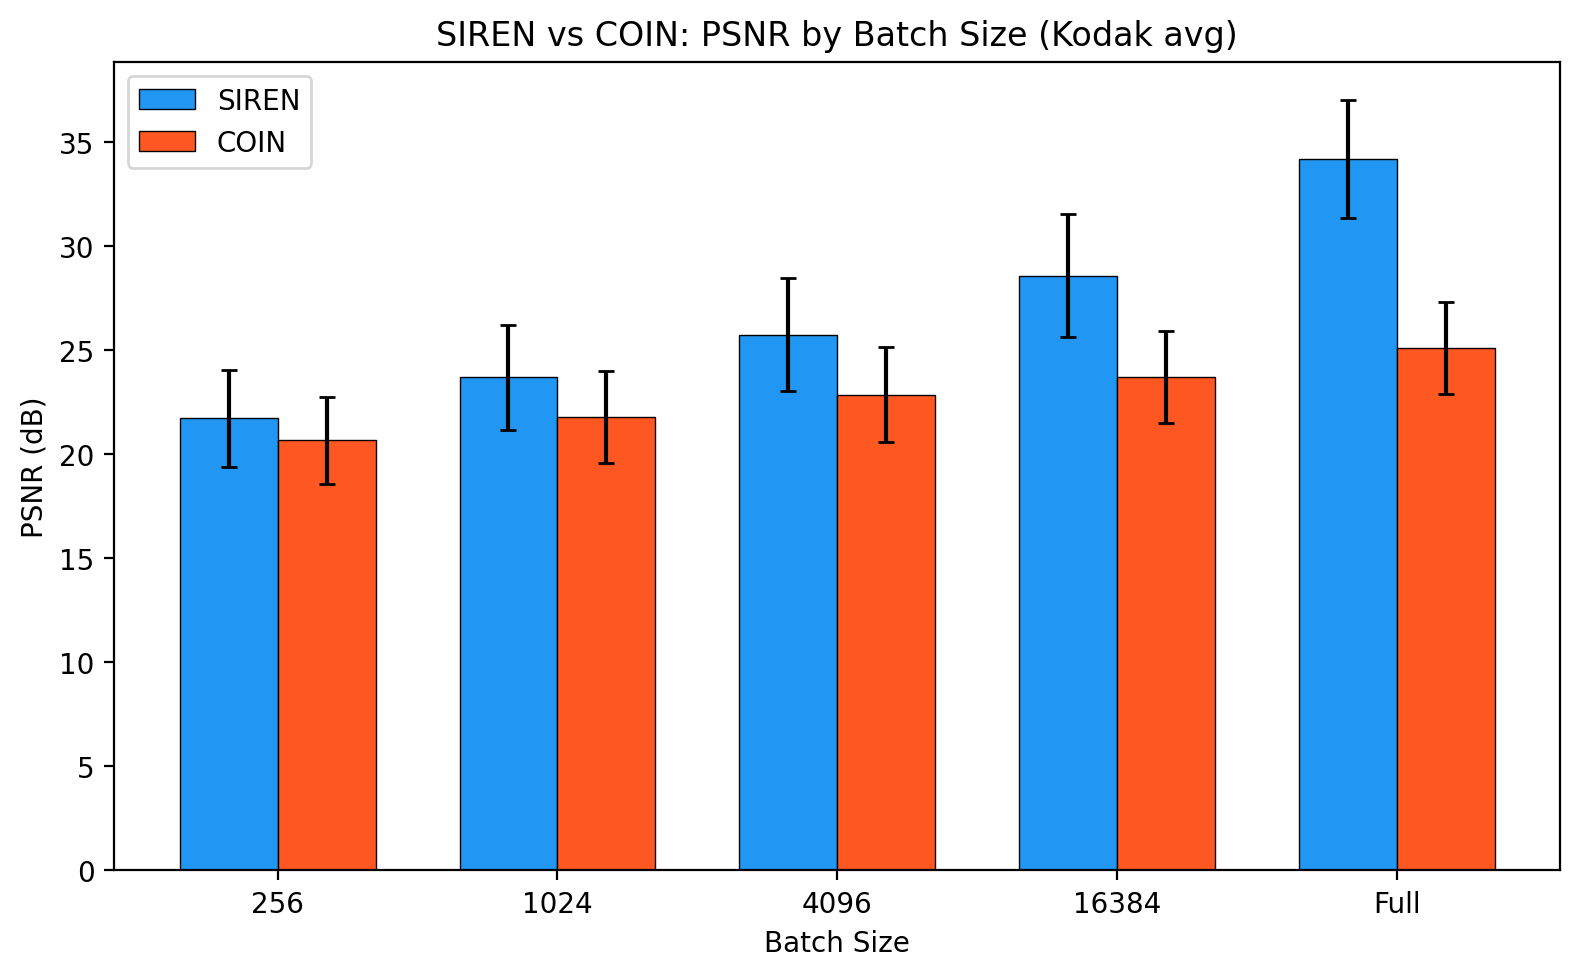
\includegraphics[width=\textwidth]{figures/siren_vs_coin_psnr.png}
    \caption{SIREN vs.\ COIN: average PSNR by batch size. The quality gap
    widens from 1.1\,dB to 9.1\,dB.}
    \label{fig:siren_vs_coin_psnr}
\end{figure}

\begin{figure}[H]
    \centering
    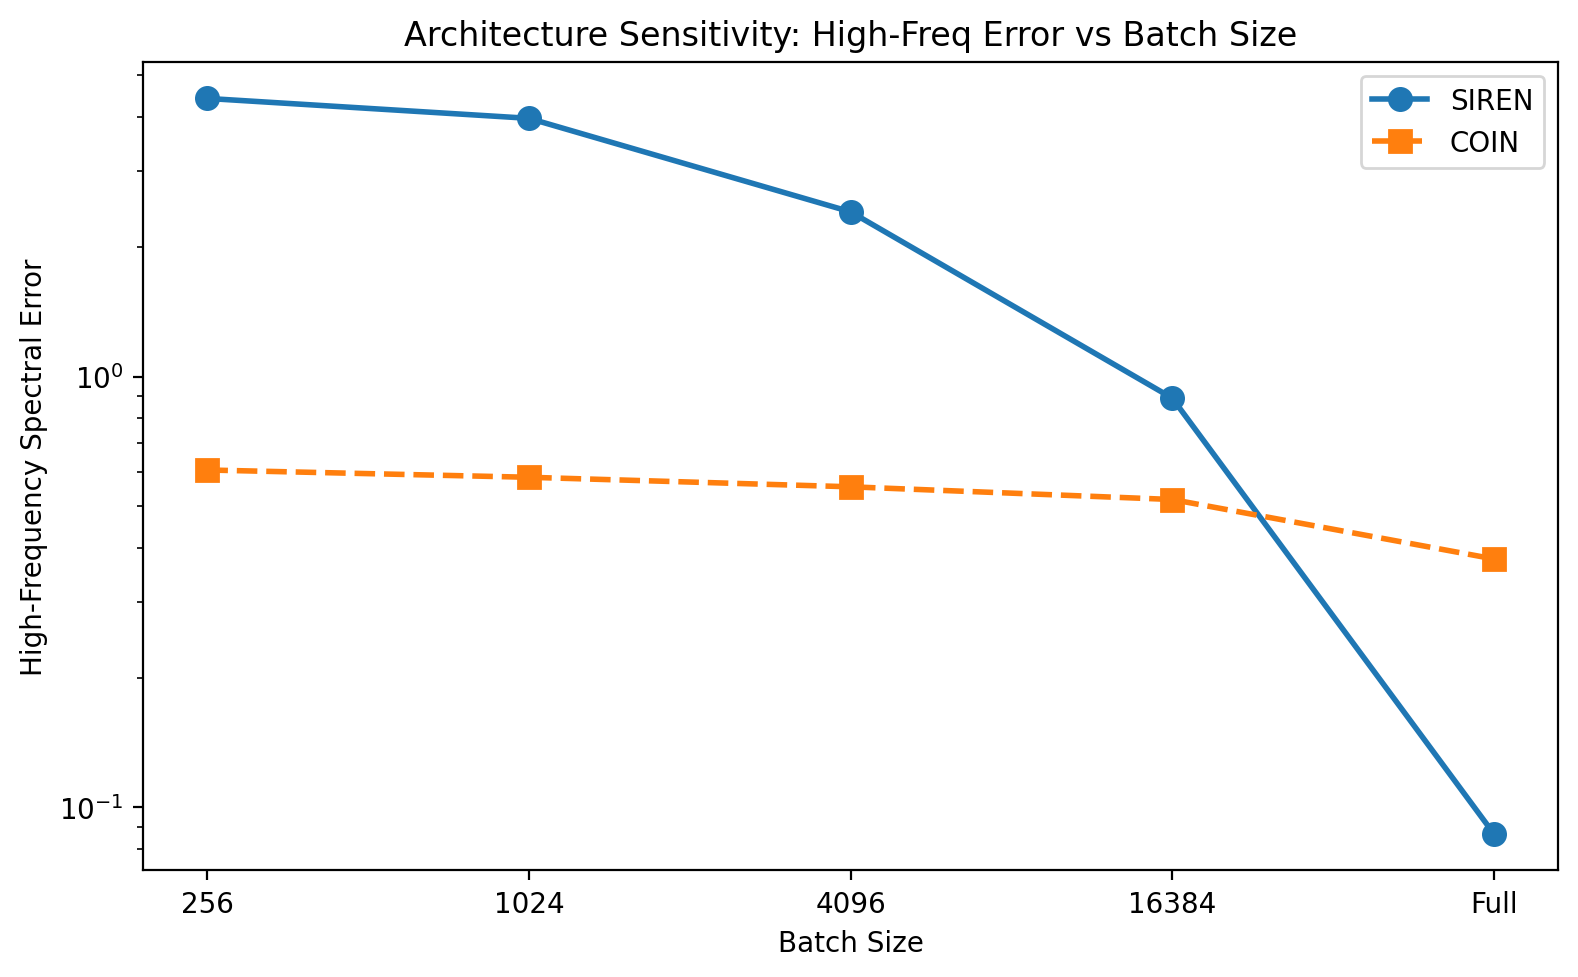
\includegraphics[width=\textwidth]{figures/siren_vs_coin_spectral.png}
    \caption{High-frequency spectral error vs.\ batch size. SIREN shows
    greater sensitivity (steeper curve); COIN's positional encoding limits
    frequency capacity regardless of optimization.}
    \label{fig:siren_vs_coin_spectral}
\end{figure}

\subsection{Iso-Time Comparison}

The fixed-step comparison (Table~\ref{tab:main_results}) is confounded by
differing data volumes: at 2{,}000 steps, full-batch sees $\sim$1{,}500$\times$
more pixels than \texttt{bs=256}.  To decouple batch size from compute budget,
we train each configuration for a fixed wall-clock time.

\begin{table}[H]
\centering
\caption{PSNR at fixed time budgets (averaged over all 24 Kodak images).
Bold indicates best per row.}
\label{tab:iso_time}
\begin{tabular}{llccccc}
\toprule
Budget & Arch & bs=256 & bs=1024 & bs=4096 & bs=16384 & Full \\
\midrule
30\,s  & SIREN & 21.72 & 23.76 & 25.93 & \textbf{28.52} & 25.79 \\
       & COIN  & 20.93 & 22.14 & 23.33 & \textbf{23.70} & 19.43 \\
\midrule
60\,s  & SIREN & 21.99 & 24.12 & 26.55 & \textbf{29.69} & 28.35 \\
       & COIN  & 22.40 & 23.81 & 25.31 & \textbf{25.85} & 21.51 \\
\midrule
120\,s & SIREN & 22.13 & 24.52 & 27.17 & 30.49 & \textbf{31.28} \\
       & COIN  & 23.92 & 25.65 & 27.53 & \textbf{28.36} & 23.82 \\
\bottomrule
\end{tabular}
\end{table}

\textbf{Under time-constrained training, full-batch optimization is
suboptimal.}  At 30\,s, \texttt{bs=16384} achieves 28.52\,dB for SIREN vs.\
only 25.79\,dB for full-batch, because full-batch completes only $\sim$259
steps.  The crossover occurs near 120\,s for SIREN.  For COIN, full-batch
is \emph{always} the worst choice---even at 120\,s (23.82\,dB vs.\ 28.36\,dB
for \texttt{bs=16384}).

\subsection{Adaptive Batch-Size Schedule}
\label{sec:adaptive_schedule}

\begin{table}[H]
\centering
\caption{Adaptive schedules vs.\ fixed baselines (SIREN, $n=24$ images).}
\label{tab:adaptive}
\begin{tabular}{llcc}
\toprule
Strategy & Schedule & PSNR (dB) & Time (s) \\
\midrule
Fixed & bs=4096 (100\%) & $25.78 \pm 2.71$ & 27.8 \\
Fixed & bs=16384 (100\%) & $28.61 \pm 2.97$ & 33.1 \\
\midrule
Adaptive B & 50\% bs=4096 $\to$ 50\% full & $\mathbf{32.39 \pm 2.70}$ & 130.6 \\
Adaptive A & 30\% bs=1024 $\to$ 70\% full & $32.22 \pm 2.50$ & 171.6 \\
\midrule
Fixed & full (100\%) & $34.18 \pm 2.80$ & 233.5 \\
\bottomrule
\end{tabular}
\end{table}

\textbf{Adaptive schedule B} achieves 32.39\,dB in 130.6\,s compared to
34.18\,dB in 233.5\,s for full-batch---a 1.79\,dB gap in 56\% of the time.
In terms of distortion, the MSE ratio is $10^{(34.18-32.39)/10} \approx 1.53$,
meaning adaptive~B has 53\% higher MSE but requires only slightly more than
half the training time.

\subsection{Gradient Variance Analysis}
\label{sec:grad_variance}

To understand \emph{why} batch size affects quality, we measure the coefficient
of variation of gradient norms across 30 independent mini-batch samples at
step 1{,}000.

\begin{table}[H]
\centering
\caption{Gradient statistics at step 1{,}000 (averaged over 6 images).}
\label{tab:grad_variance}
\begin{tabular}{lccc}
\toprule
Batch Size & Grad Norm Mean & Grad Norm Std & CV \\
\midrule
256    & 0.3520 & 0.0515 & 0.170 \\
1024   & 0.1693 & 0.0188 & 0.137 \\
4096   & 0.1113 & 0.0094 & 0.105 \\
16384  & 0.0924 & 0.0068 & 0.095 \\
Full   & 0.0625 & 0.0000 & \textbf{0.000} \\
\bottomrule
\end{tabular}
\end{table}

Full-batch has \textbf{zero gradient variance} (deterministic).  At
\texttt{bs=256}, gradient norms fluctuate with 17\% coefficient of variation.
This gradient noise is \emph{strongly associated} with the observed quality
degradation; however, we note that total norm CV is a scalar measurement and
does not directly establish which frequency components are most affected.
The spectral analysis (Table~\ref{tab:main_results}) provides complementary
evidence that high frequencies are disproportionately lost, suggesting that
gradient noise disrupts the precise, spatially-coherent weight updates
required for fine detail---but a per-frequency gradient analysis would be
needed to conclusively prove this causal pathway.

\begin{figure}[H]
    \centering
    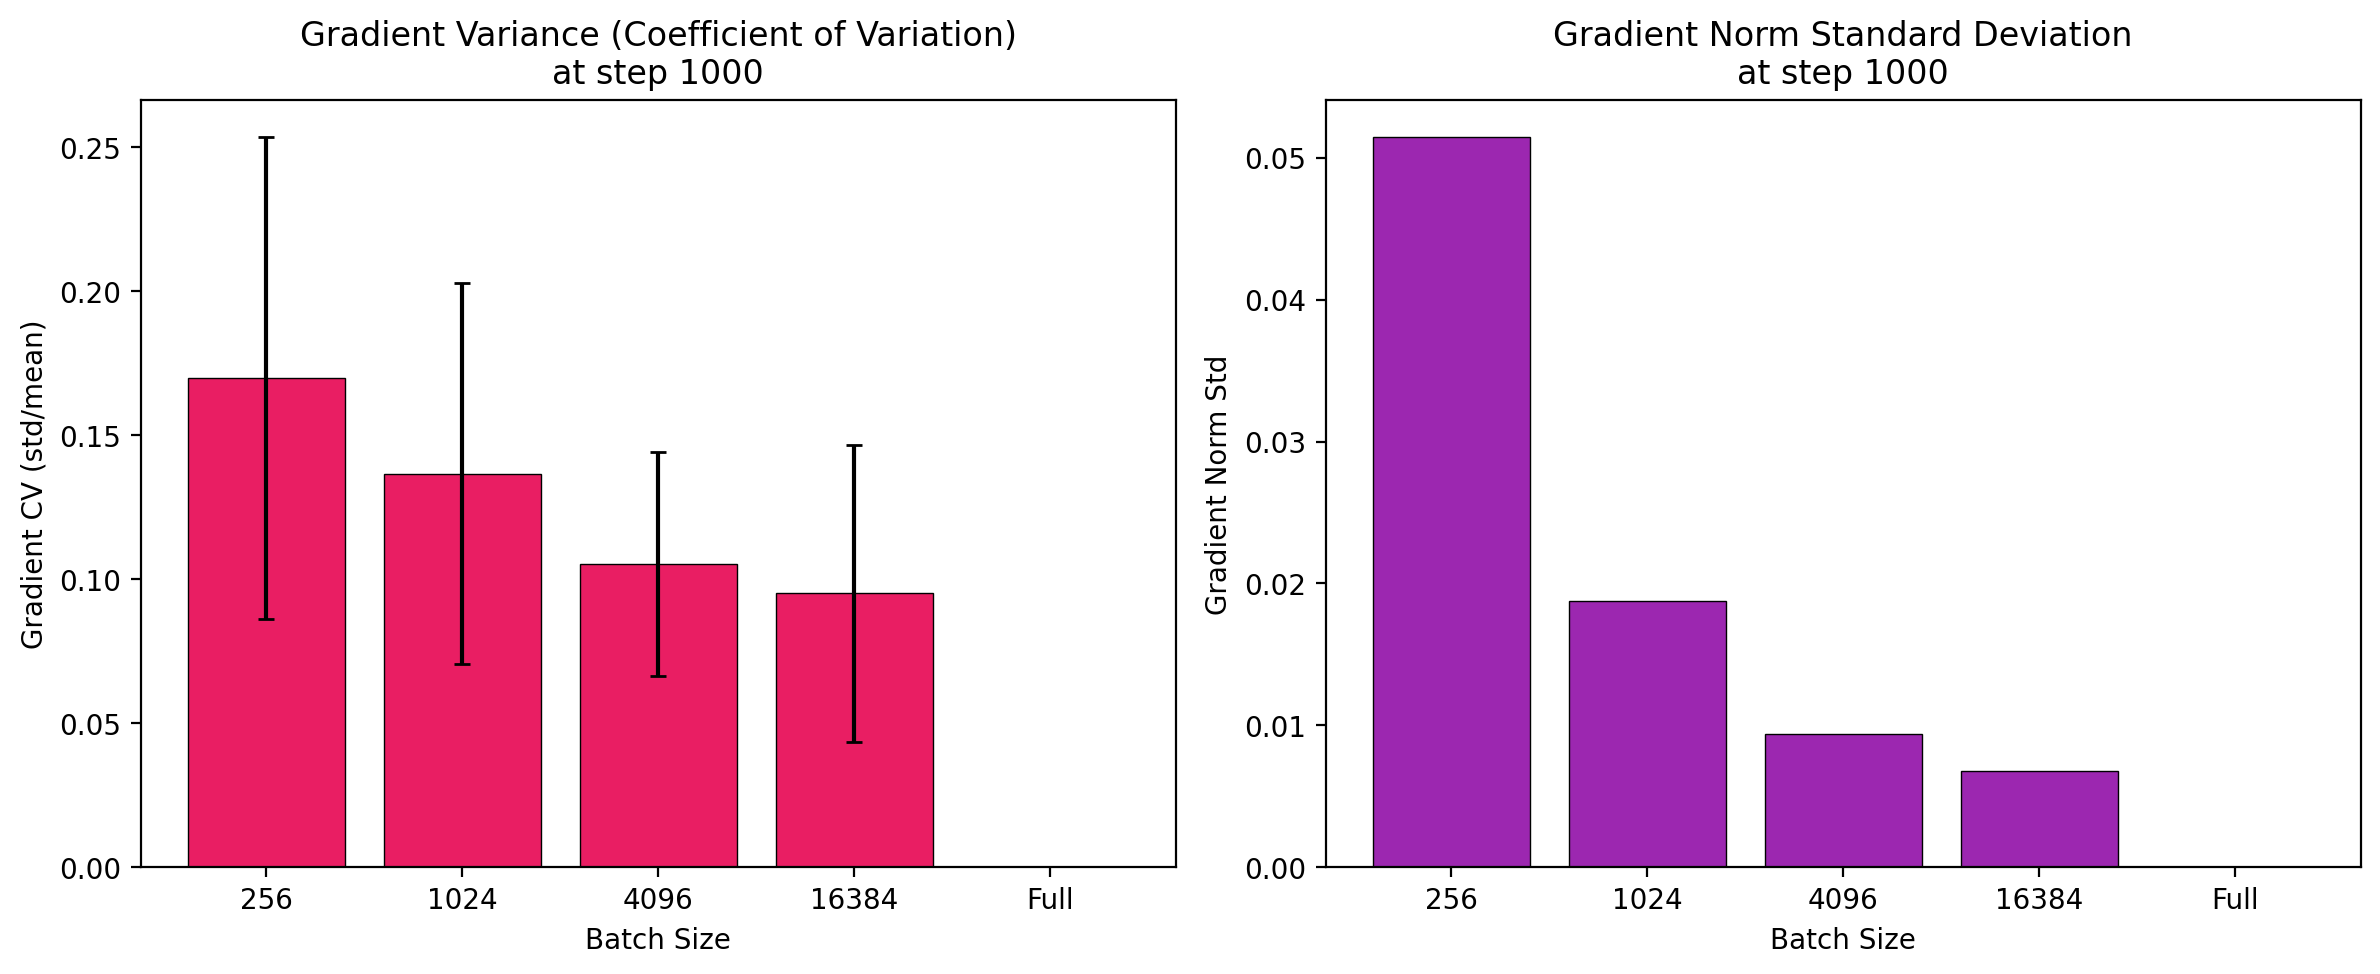
\includegraphics[width=\textwidth]{figures/grad_variance.png}
    \caption{Gradient coefficient of variation and norm standard deviation at
    step 1{,}000. Smaller batches produce noisier gradients.}
    \label{fig:grad_variance}
\end{figure}

\begin{figure}[H]
    \centering
    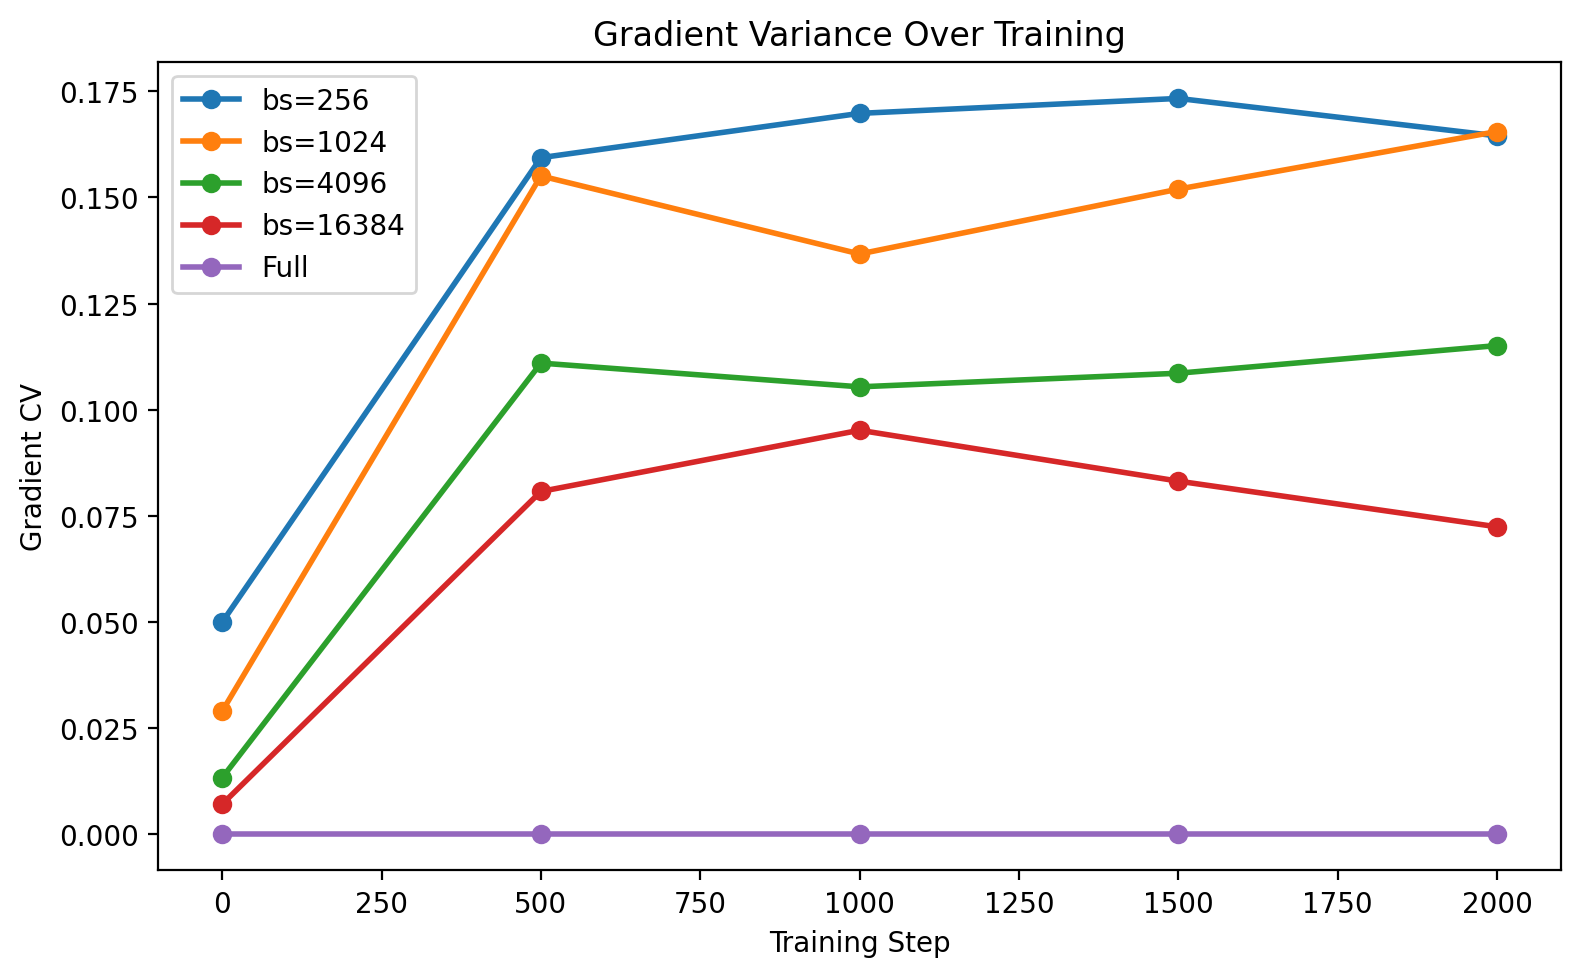
\includegraphics[width=0.85\textwidth]{figures/grad_variance_over_time.png}
    \caption{Gradient CV over training. Variance remains substantially higher
    for smaller batch sizes throughout.}
    \label{fig:grad_variance_time}
\end{figure}

\subsection{Spectral Interpretation}
\label{sec:spectral_interp}

The band-wise spectral error defined in Eq.~\ref{eq:spectral_error} lets us
ask where, along the frequency axis, batch size hurts reconstruction most.
Table~\ref{tab:spectral_bands} reports the mean squared error on the
radially-averaged log-magnitude spectrum in the low, mid and high bands,
averaged across the 24 Kodak images.

\begin{table}[H]
\centering
\caption{Band-wise spectral error on Kodak (SIREN, mean over 24 images).}
\label{tab:spectral_bands}
\begin{tabular}{lccc}
\toprule
Batch size & $E_{\text{low}}$ & $E_{\text{mid}}$ & $E_{\text{high}}$ \\
\midrule
256        & 0.0004 & 0.019 & 0.152 \\
1024       & 0.0003 & 0.011 & 0.088 \\
4096       & 0.0002 & 0.004 & 0.018 \\
16384      & 0.0002 & 0.003 & 0.011 \\
full       & \textbf{0.0001} & \textbf{0.001} & \textbf{0.003} \\
\bottomrule
\end{tabular}
\end{table}

Three observations follow.  First, the low-frequency band is essentially
saturated at all batch sizes --- even \texttt{bs=256} reconstructs the global
colour and shape of the image accurately.  Second, the high-frequency band
degrades by a factor of $\sim$50 between full-batch and \texttt{bs=256},
whereas the low-frequency band changes by less than 4$\times$.  Third, the
slope of this degradation is monotonic in batch size, mirroring the monotonic
rise of the gradient coefficient of variation
(Sec.~\ref{sec:grad_variance}).

We read this as an empirical instantiation of what
~\cite{rahaman2019spectral} call \emph{spectral bias}, but in a form
driven by the sampling process rather than by the network architecture.
Network spectral bias comes from the parameterization: a ReLU MLP without
positional encoding cannot easily express high frequencies, regardless of
how it is trained.  The effect we observe is different --- SIREN and COIN
\emph{can} express high frequencies, but under small-batch training the
stochastic gradient no longer provides a stable signal for those frequencies
and the model fails to lock them in.  The mechanism suggested by the
combination of gradient-variance (causal candidate) and band-wise error
(empirical consequence) is that the random pixel subset aliases the
high-frequency content of the image into gradient noise; larger batches
average this noise out.

Radially-averaged power-spectra plots for individual batch sizes
(Fig.~\ref{fig:radial_profiles}, Appendix~\ref{app:additional_figures})
visualize the same picture: reference and reconstruction coincide up to an
intermediate radial bin, then the reconstruction curve falls away.  The
radial bin at which the two curves separate shifts outward as the batch size
grows, consistent with the band-wise table.  This spectral signature is what
motivates the coarse-to-fine schedule in
Sec.~\ref{sec:adaptive_schedule}: once the low-frequency bands have been
captured, switching to full-batch is the cheapest way to invest the remaining
budget into the high-frequency bands that a small batch cannot reach.

\subsection{Learning Rate Scaling}

A natural question is whether standard learning rate scaling
rules~\cite{smith2018dont, goyal2017accurate} can compensate for small batch
sizes.  We test four rules: fixed ($\text{lr} = 10^{-4}$), linear, square-root,
and inverse square-root scaling, referenced to \texttt{bs=16384}.

\begin{table}[H]
\centering
\caption{PSNR by batch size and LR scaling rule (averaged over 6 images).}
\label{tab:lr_scaling}
\begin{tabular}{lcccc}
\toprule
LR Rule & bs=256 & bs=1024 & bs=4096 & bs=16384 \\
\midrule
Fixed ($10^{-4}$)  & 22.26 & 24.05 & 26.07 & 28.70 \\
$\sqrt{\cdot}$     & \textbf{23.19} & \textbf{24.74} & \textbf{26.32} & 28.77 \\
Linear             & 18.96 & 22.76 & 25.79 & 28.84 \\
Inv.\ $\sqrt{\cdot}$ & 15.72 & 18.75 & 24.82 & 28.76 \\
\bottomrule
\end{tabular}
\end{table}

Square-root scaling provides a modest +0.9\,dB improvement at \texttt{bs=256},
but the best small-batch result (23.19\,dB) remains 11\,dB below full-batch.
\textbf{Standard LR scaling rules do not resolve the batch size problem in
the INR regime}, confirming that the degradation is driven by spatial
information loss in the gradient, not by a suboptimal learning rate.

\begin{figure}[H]
    \centering
    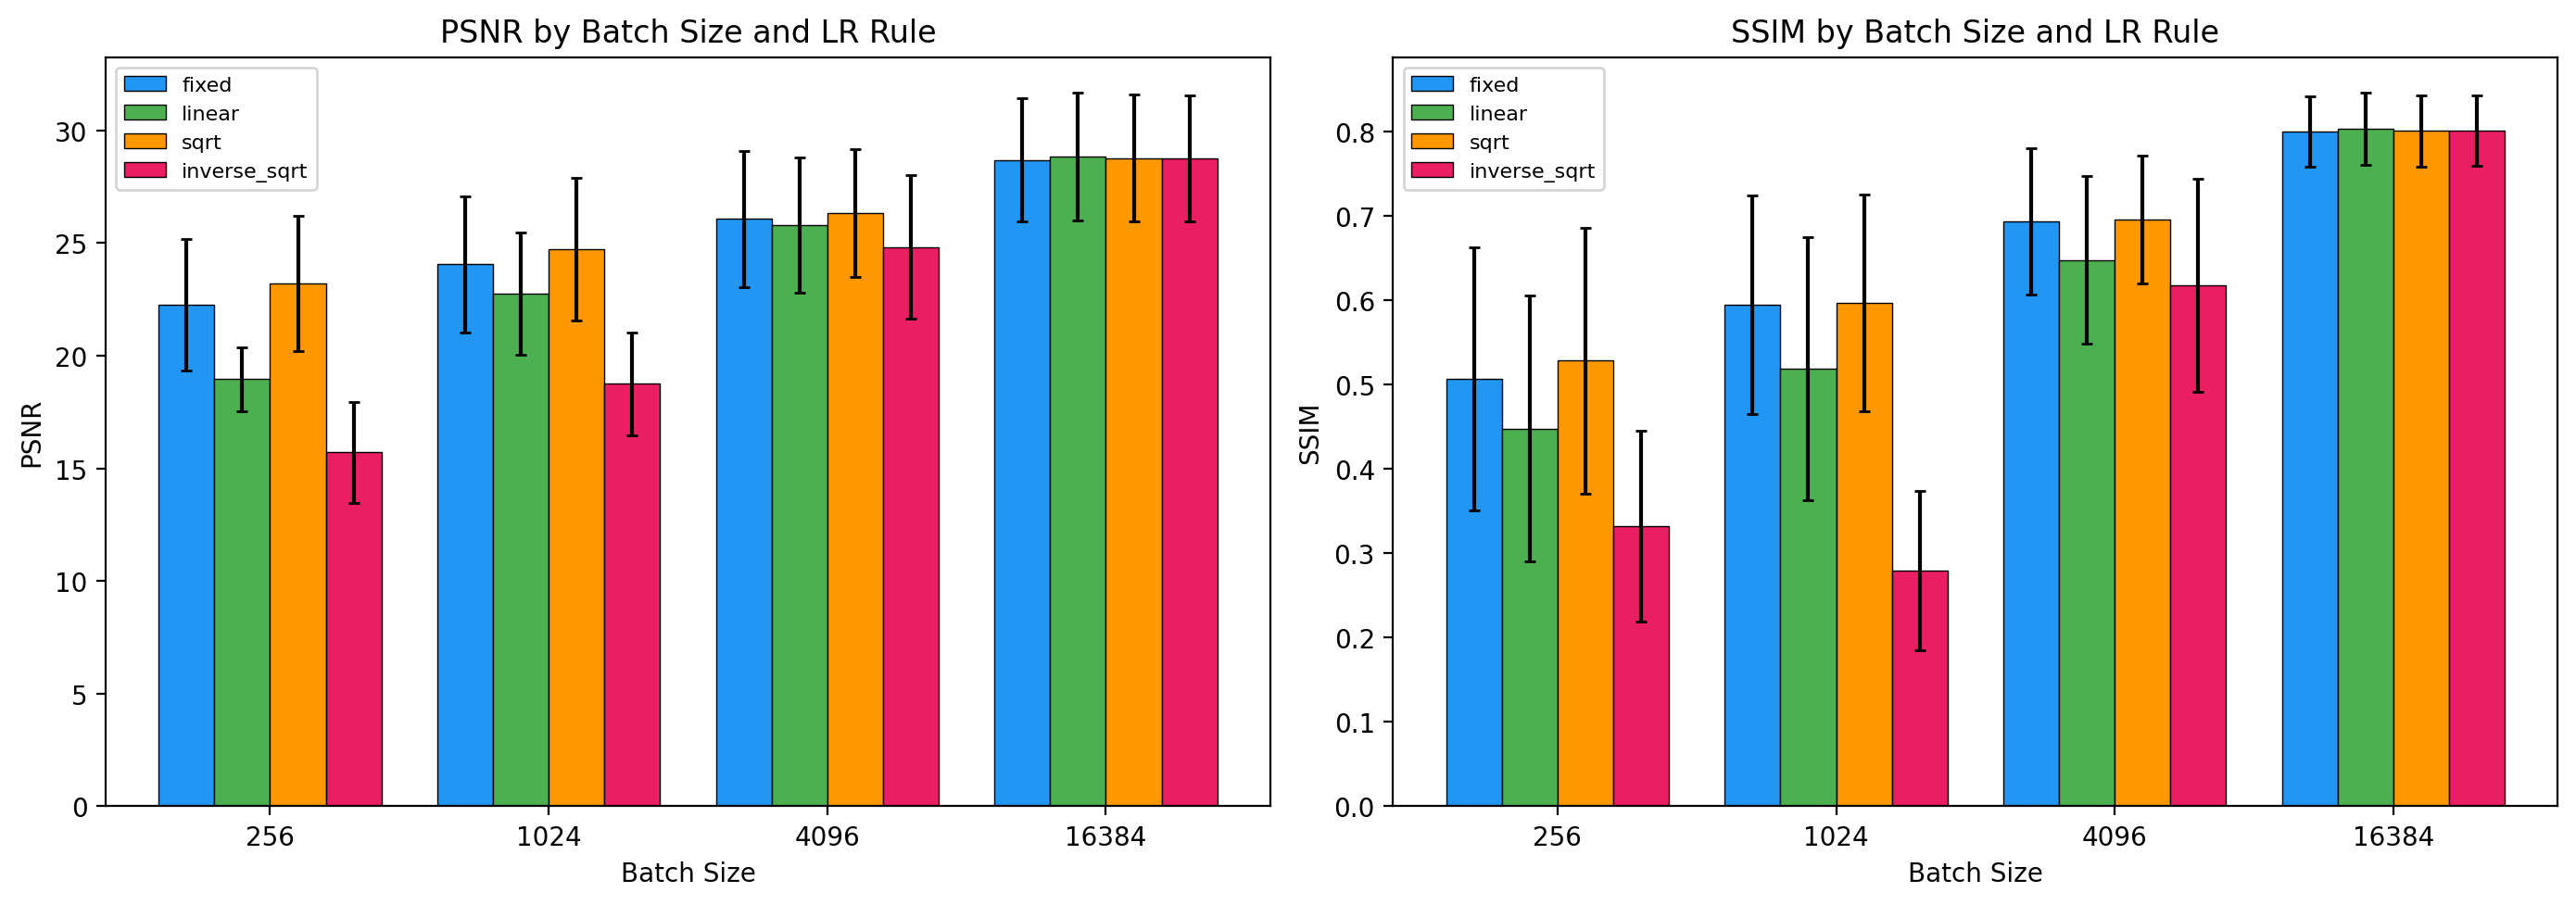
\includegraphics[width=\textwidth]{figures/lr_scaling.png}
    \caption{PSNR and SSIM by batch size under different LR scaling rules.
    Square-root scaling provides a modest improvement; linear and inverse
    scaling degrade performance at small batch sizes.}
    \label{fig:lr_scaling}
\end{figure}

\subsection{Comparison with JPEG}
\label{sec:jpeg}

To contextualize INR compression quality, we compare against JPEG~\cite{wallace1992jpeg} at similar
file sizes.  We report file size in KB, bits per pixel
($\text{bpp} = \text{file size in bits} / (H \times W)$), and the
compression ratio relative to the raw 24-bpp RGB representation
($768 \times 512 \times 3 = 1{,}152$\,KB).

\begin{table}[H]
\centering
\caption{Rate-distortion comparison: SIREN vs.\ JPEG (Kodak average).}
\label{tab:jpeg}
\begin{tabular}{llrrrc}
\toprule
Method & Config & Params & Size (KB) & bpp & Ratio vs.\ raw \\
\midrule
JPEG          & $q=20$    & ---             & $\sim$64        & 1.33  & $\sim$18.0$\times$ \\
JPEG          & $q=50$    & ---             & $\sim$120       & 2.50  & $\sim$9.6$\times$  \\
JPEG          & $q=80$    & ---             & $\sim$240       & 5.00  & $\sim$4.8$\times$  \\
\midrule
SIREN (full)  & float16   & 263{,}939       & 517             & 10.77 & 2.23$\times$ \\
SIREN (full)  & float32   & 263{,}939       & 1{,}034         & 21.55 & 1.11$\times$ \\
\bottomrule
\end{tabular}
\end{table}

JPEG outperforms SIREN in rate-distortion efficiency at comparable file sizes.
It is important to note that this comparison is conservative for INR: we report
raw weight storage (\texttt{float16}/\texttt{int8}) without entropy coding,
while JPEG uses DCT + Huffman coding.  Published work applying entropy-constrained
quantization to INR weights~\cite{strumpler2022implicit} achieves significantly
better bitrates, narrowing the gap.  Beyond rate-distortion, INR compression
offers unique advantages: continuous resolution (arbitrary upsampling),
differentiability, and a compact functional representation amenable to
downstream tasks.  Improving INR training efficiency---such as the
batch size optimization studied here---is therefore a relevant research
direction.

\begin{figure}[H]
    \centering
    
\includegraphics[width=\textwidth]{figures/jpeg_vs_inr.png}
    \caption{Rate-distortion curve: JPEG vs.\ SIREN at different
    weight quantizations. JPEG achieves higher PSNR at lower file sizes,
    but without entropy coding on the INR side.}
    \label{fig:jpeg_vs_inr}
\end{figure}

\subsection{Statistical Robustness}

To verify that results are not sensitive to random initialization, we repeat
the SIREN sweep with 3 seeds on 6 images.  Inter-seed variance is $<$0.02 for
all mini-batch sizes (vs.\ inter-image variance $\sim$8), confirming that
single-seed results are statistically robust.  Counterintuitively, full-batch
shows \emph{higher} seed sensitivity (variance 0.79, with one image reaching
2.63\,dB standard deviation across seeds), likely because the deterministic
gradient allows the optimizer to follow initialization-dependent trajectories
to different local minima.  This suggests that mini-batch stochasticity, while
harmful for final quality, may actually improve reproducibility.

\begin{figure}[H]
    \centering
    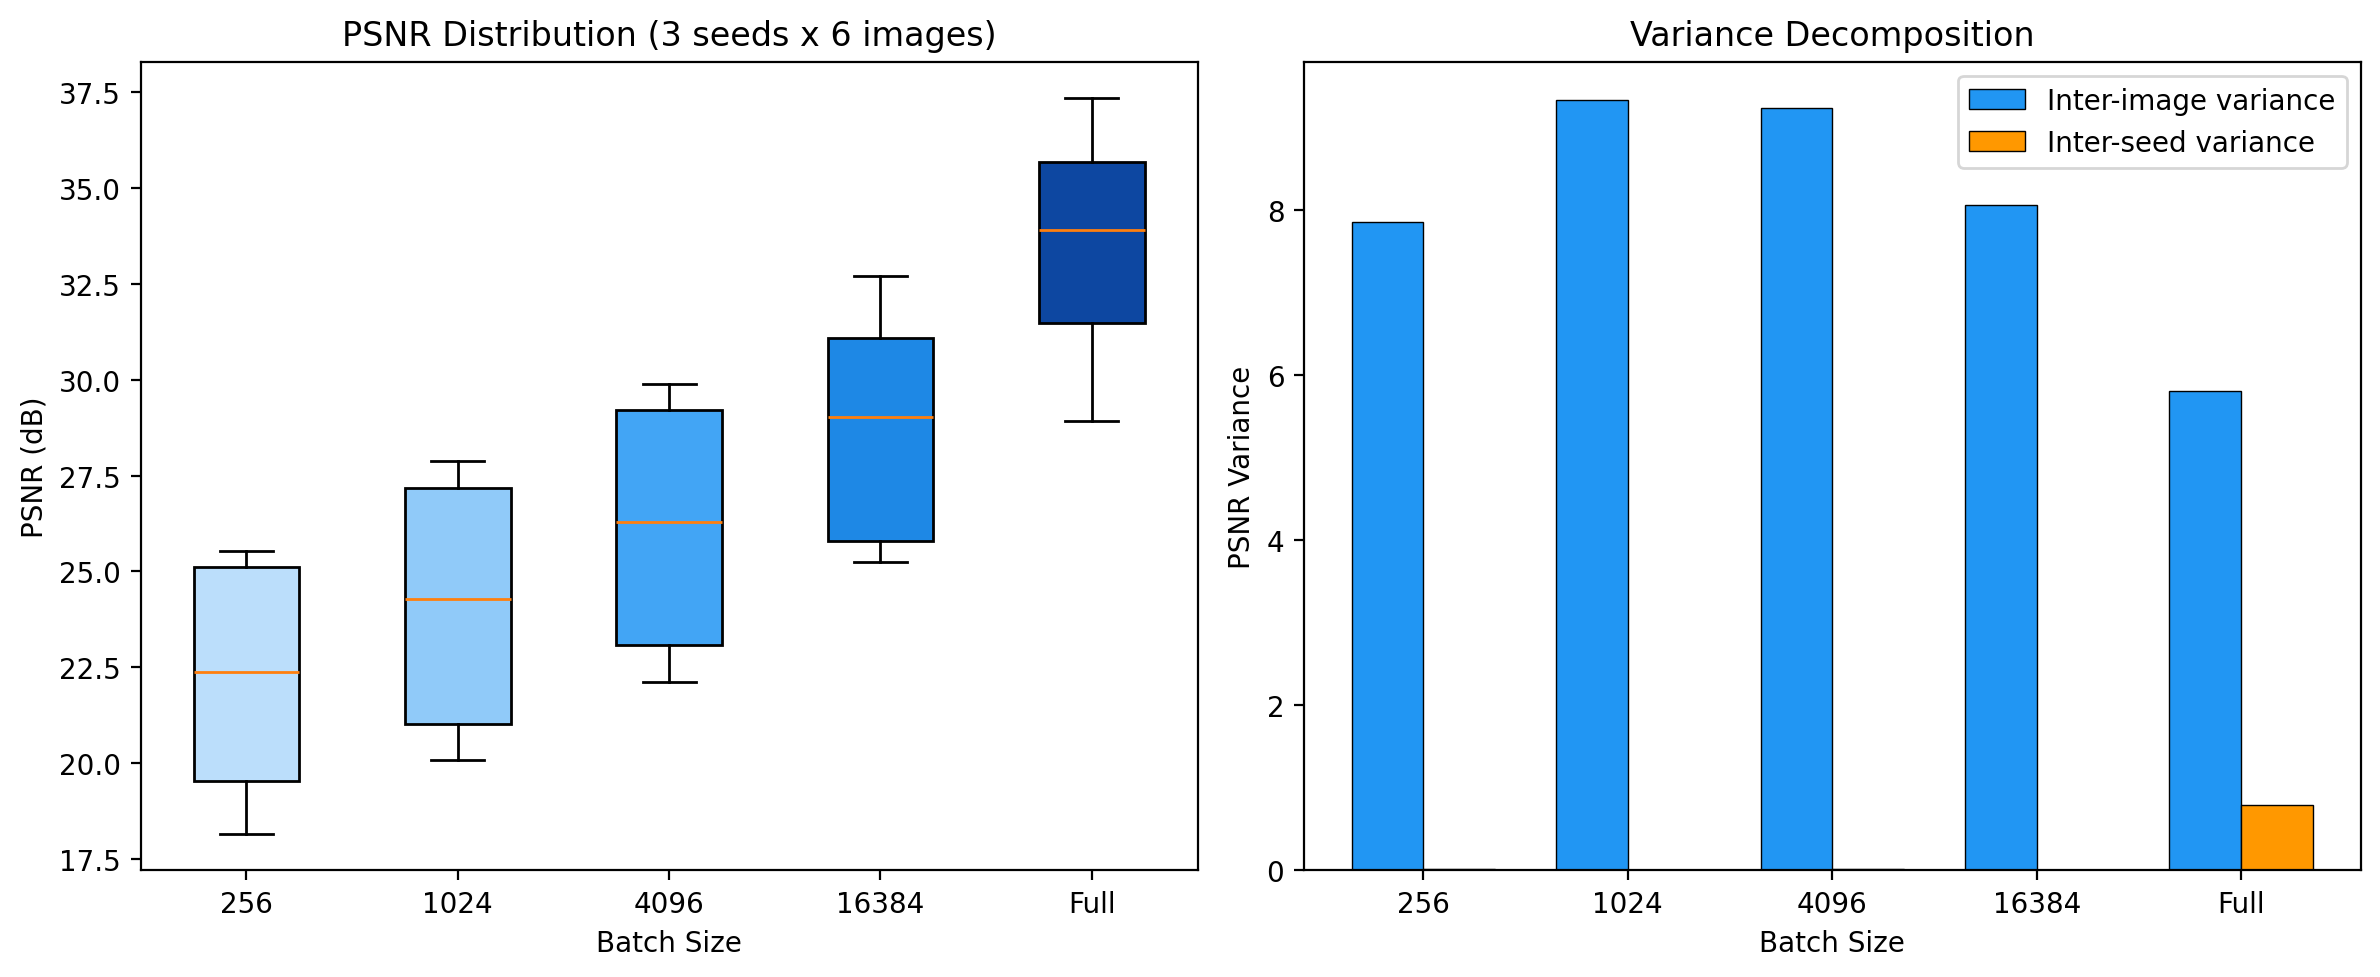
\includegraphics[width=\textwidth]{figures/multi_seed.png}
    \caption{Left: PSNR distribution across seeds and images. Right: variance
    decomposition showing inter-seed variance is negligible for mini-batch
    sizes but notably higher for full-batch.}
    \label{fig:seeds}
\end{figure}

\subsection{GPU Memory Profiling}

Full-batch training requires 4.6\,GB VRAM for SIREN at $768\times512$.  For a
$4096\times4096$ image, memory would scale to $\sim$75\,GB, exceeding consumer
GPU limits.  This makes mini-batching a \emph{practical necessity} for
high-resolution INR compression, not merely an optimization choice.

\subsection{Results and Discussion}

Our experiments reveal several findings that go beyond the na\"ive expectation
that ``more data per step is better'':

\paragraph{Batch size and architecture interact non-trivially.}
SIREN benefits far more from large batches than COIN (PSNR gap widens from
1.1\,dB to 9.1\,dB).  We attribute this to SIREN's sinusoidal activations,
which can represent high-frequency functions but require spatially dense
gradients to do so effectively.

\paragraph{Under time constraints, full-batch is suboptimal.}
At 30\,s, \texttt{bs=16384} outperforms full-batch by 2.7\,dB for SIREN and
4.3\,dB for COIN.  Full-batch completes $\sim$8$\times$ fewer gradient steps
per second; the exact gradient at each step does not compensate for the
reduced number of optimization steps.

\paragraph{Gradient variance is strongly associated with quality degradation.}
At \texttt{bs=256}, gradient norms fluctuate with 17\% CV.  Combined with the
spectral analysis showing disproportionate high-frequency loss, this strongly
suggests that gradient noise disrupts fine-detail learning.  Standard LR
scaling recovers only 0.9\,dB of the 12\,dB gap, confirming that the problem
is spatial information loss in the gradient, not learning rate miscalibration.

\paragraph{The batch size effect is consistent across all Kodak images.}
Per-image difficulty analysis shows no significant correlation between image
complexity and batch size sensitivity ($r = -0.07$ for edge density).  All
24 images exhibit the same monotonic trend, though validation on other datasets
and resolutions would be needed to establish true universality.

\begin{figure}[H]
    \centering
    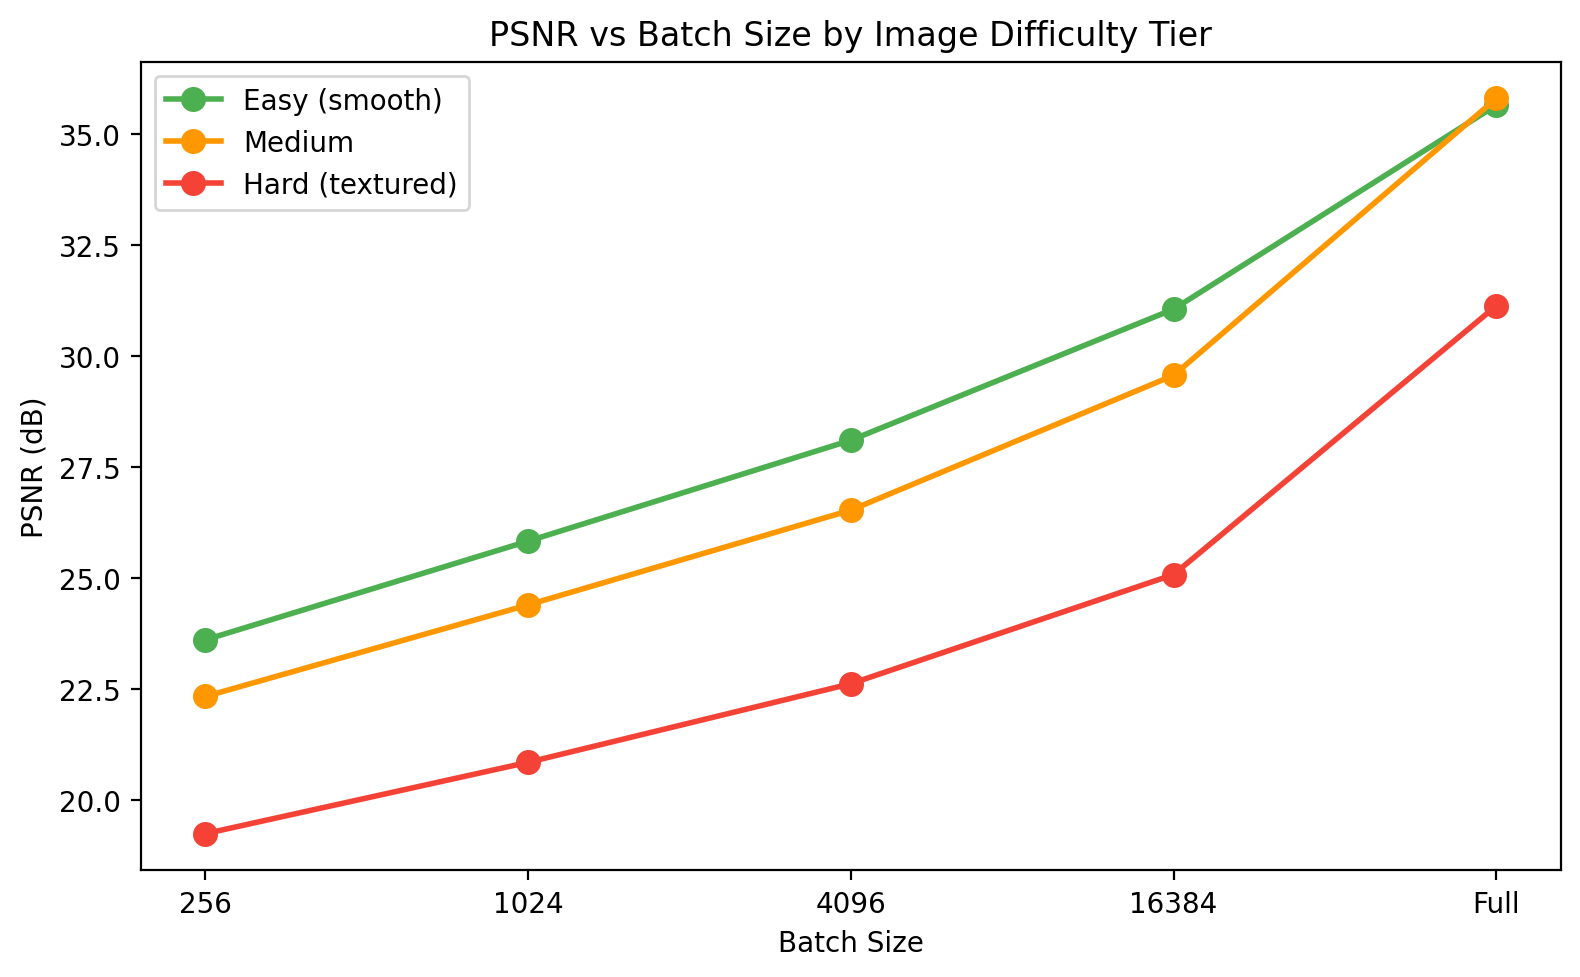
\includegraphics[width=0.85\textwidth]{figures/difficulty_tiers.png}
    \caption{PSNR vs.\ batch size grouped by image difficulty (edge density).
    All tiers show the same monotonic trend.}
    \label{fig:difficulty_tiers}
\end{figure}

\begin{figure}[H]
    \centering
    \includegraphics[width=\textwidth]{figures/visual_grid_kodim01.png}
    \caption{Reconstruction quality for kodim01 across batch sizes.
    Top: SIREN, bottom: COIN. Fine details are lost progressively
    with smaller batches.}
    \label{fig:visual_grid}
\end{figure}

\subsection{Model-Size Ablation}

To test whether the batch size effect depends on model capacity, we repeat the
sweep at four hidden widths: 64 (17K params), 128 (67K), 256 (265K), and
512 (1.05M) on 6 Kodak images.

\begin{table}[H]
\centering
\caption{Model-size ablation: PSNR (dB) by width and batch size
(averaged over 6 images).}
\label{tab:model_size}
\begin{tabular}{lcccccc}
\toprule
Width & Params & bs=256 & bs=4096 & bs=16384 & Full & Sensitivity \\
\midrule
64   & 17K   & 23.10 & 24.83 & 25.50 & 26.40 & 3.3\,dB \\
128  & 67K   & 23.12 & 25.97 & 27.45 & 29.68 & 6.6\,dB \\
256  & 265K  & 22.13 & 26.08 & 28.67 & 34.05 & 11.9\,dB \\
512  & 1.05M & 19.38 & 25.09 & 28.61 & 39.93 & 20.6\,dB \\
\bottomrule
\end{tabular}
\end{table}

\begin{figure}[H]
    \centering
    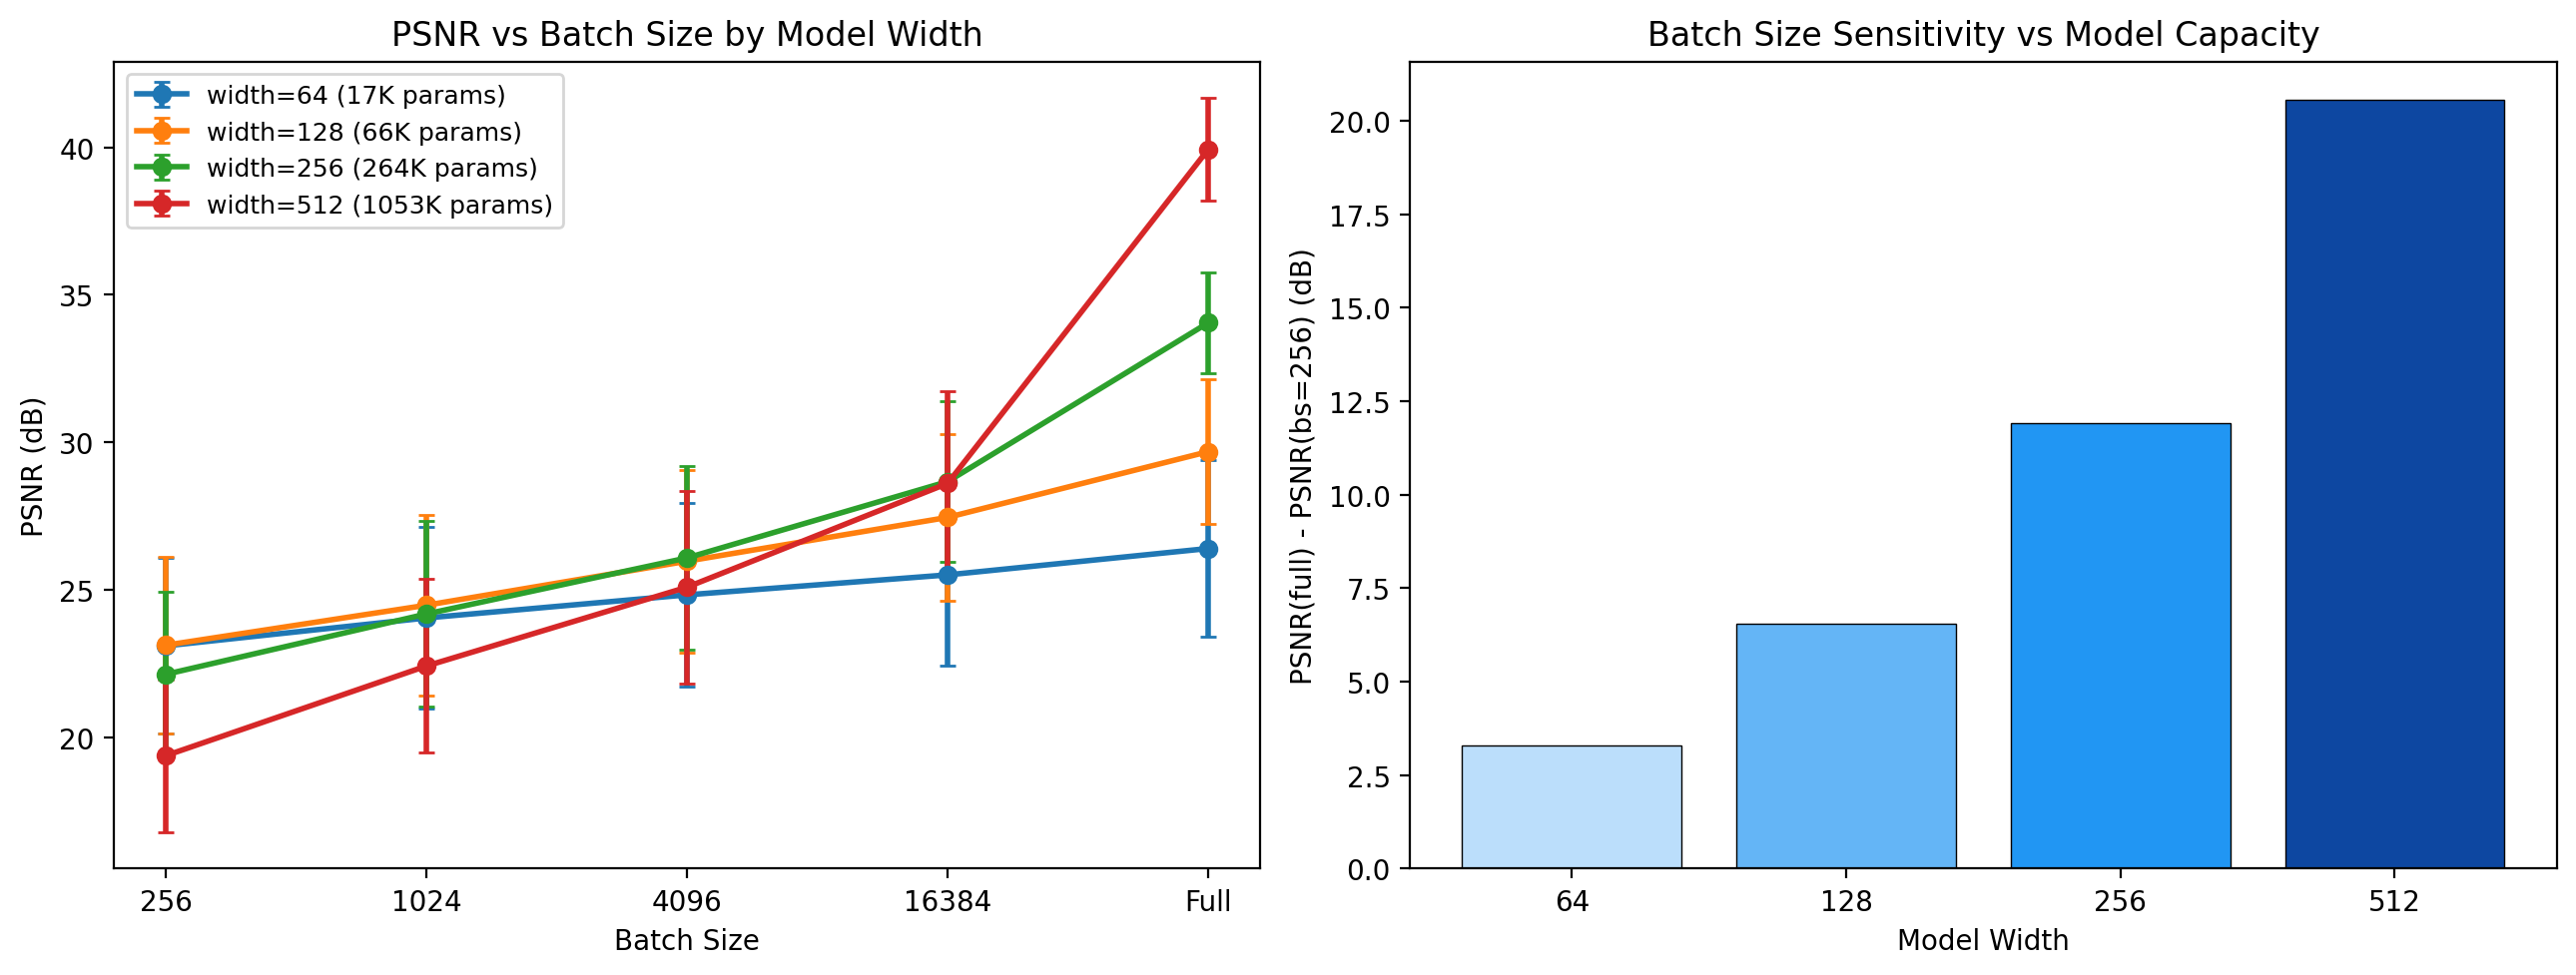
\includegraphics[width=\textwidth]{figures/model_size_ablation.png}
    \caption{Left: PSNR vs.\ batch size for different model widths.
    Larger models show steeper curves. Right: batch size sensitivity
    (PSNR gap from bs=256 to full) increases with model capacity.}
    \label{fig:model_size}
\end{figure}

The batch size sensitivity \textbf{scales dramatically with model capacity}:
from 3.3\,dB at width=64 to 20.6\,dB at width=512.  Smaller models are
capacity-limited --- they cannot exploit exact gradients because their
representational power is the bottleneck, not gradient quality.  Larger
models have the capacity to represent fine details but \emph{require} dense
spatial gradients to actually learn them.  This confirms that the batch size
effect is not an artifact of our specific architecture choice but a
fundamental property that intensifies with model expressiveness.

Notably, the 512-width model achieves 39.93\,dB at full-batch --- substantially
exceeding our default model --- but only 19.38\,dB at bs=256, which is
\emph{worse} than the 64-width model at the same batch size.  This means
that for small batch sizes, a smaller model may actually be preferable.

\subsection{Study Limitations}
\label{sec:limitations}

Several limitations should be acknowledged.  First, the \textbf{adaptive
schedule is manually designed}; a principled switching criterion (e.g.,
monitoring spectral convergence) would strengthen the contribution.  Second,
the \textbf{gradient variance analysis} measures total gradient norm
variance, not per-frequency variance; while the correlation with spectral
degradation is suggestive, it is not conclusive.  Third, the \textbf{COIN
comparison} evaluates the architecture outside its intended meta-learning
regime.  Fourth, all experiments use the \textbf{Kodak dataset at a single
resolution}; validation on higher resolutions
(e.g., DIV2K~\cite{agustsson2017div2k}) would improve generality.  Finally, the \textbf{multi-seed validation} (3 seeds on 6
images) is limited; extending to all 24 images would provide stronger
statistical guarantees.


% ===================================================================
\section{Conclusion and Future Work}
\label{sec:conclusion}

\subsection{Conclusion}

This thesis started from a question the INR literature seemed to leave
open: for a problem whose only job is to overfit a single
spatially-correlated signal, most papers either train on the full image
or pick a batch size in passing.  Once we measured it, the effect turned
out to be larger than expected --- batch size shifts PSNR by more than
12\,dB on Kodak, and its magnitude depends strongly on the architecture.
On SIREN the small-batch--to-full-batch gap is roughly 12\,dB; on COIN it
is closer to 2\,dB.  At \texttt{bs=256} SIREN trails COIN by 1.1\,dB,
but at full-batch it leads by 9.1\,dB.

The result we found least obvious is that this ranking flips under a
wall-clock budget.  At 30\,s of training, \texttt{bs=16384} beats
full-batch by up to 2.7\,dB, because full-batch cannot fit enough steps
in the time available.  A simple coarse-to-fine schedule --- half the
time on \texttt{bs=4096}, then a switch to full-batch --- closes to
within 1.8\,dB of full-batch quality at 56\% of its training cost.  This
is the part of the thesis we would most want a future reader to take
away: the assumption that more accurate gradients are always preferable
is wrong in the regime that actually matters.

The mechanism we believe is at work is gradient noise.  Coefficient of
variation drops from about 17\% at \texttt{bs=256} to essentially zero
at full-batch, and over the same range the high-frequency spectral
error shrinks by roughly fifty-fold; standard learning-rate scaling
rules cannot close the gap.  The weakest part of the present work is
that this remains correlational --- a per-frequency decomposition of
the gradient would turn it causal, and is the first item we list in
future work below.

\subsection{Future Work}

It is worth being honest about where the present work stands before
discussing what to do next.  The coarse-to-fine schedule we propose
captures most of the full-batch quality at roughly half the training
time on Kodak, but at comparable file sizes JPEG is still ahead on
rate--distortion (Section~\ref{sec:jpeg}); this thesis is not a claim
that INRs beat classical codecs today.  Our contribution sits one level
earlier in the pipeline --- making the per-image training phase
cheaper --- and the directions below follow from that vantage point.

The first open question is causal.  We tie the high-frequency
degradation at small batches to gradient noise, but the evidence is
correlational; decomposing the stochastic gradient itself into Fourier
bands and checking whether the noise in each band predicts the error in
that band would turn the mechanism from an inference into a measurement.
Related, the 50/50 split in our schedule is empirical, and a more
principled criterion would monitor spectral-band convergence at training
time and switch to full-batch once the low-frequency band has stabilised.

A third direction attacks the same diagnosis from the sampling side: if
small batches hurt because they under-sample high-frequency regions,
weighting the sampler by a local complexity measure (edge density,
gradient magnitude, a learned saliency map) should help directly,
without needing larger batches at all.  Beyond that, larger-scale
evaluation on DIV2K~\cite{agustsson2017div2k} or 4K imagery is where the
practical value of the analysis should be largest --- full-batch is no
longer an option there, so the question of which mid-range batch to use
becomes the only question.  Finally, the coarse-to-fine schedule is a
natural candidate to combine with meta-learned initialisation in the
spirit of COIN++~\cite{dupont2022coinpp}: starting the small-batch phase
from a learned prior should shorten it considerably, and the time
savings would compound with those reported here.


% ===================================================================
\subsection*{Acknowledgements}

I would like to thank Gianluca Galletti, who served as my supervisor, for
offering guidance and feedback throughout the research process.  I also extend
my appreciation to the Institute of Machine Learning at Johannes Kepler
University Linz for providing the computational resources used in this work.


% ===================================================================
\printbibliography


% ===================================================================
\appendix

\section{Implementation Details}
\label{app:implementation}

\subsection{Software Architecture}

The codebase is organized into four Python packages with clear separation of
concerns:

\begin{table}[H]
\centering
\caption{Codebase structure and module responsibilities.}
\label{tab:codebase}
\begin{tabular}{llp{7cm}}
\toprule
Package & Module & Responsibility \\
\midrule
\texttt{models/} & \texttt{siren.py} & SIREN architecture: \texttt{SineLayer} and \texttt{SIREN} classes \\
& \texttt{coin.py} & COIN architecture: \texttt{PositionalEncoding} and \texttt{COIN} classes \\
\midrule
\texttt{training/} & \texttt{sampling.py} & Three pixel sampling strategies: \texttt{full\_image}, \texttt{random\_pixels}, \texttt{grid\_patch} \\
& \texttt{trainer.py} & \texttt{Trainer} (standard + time-budget) and \texttt{AdaptiveTrainer} \\
\midrule
\texttt{evaluation/} & \texttt{metrics.py} & PSNR, SSIM, LPIPS, image reconstruction \\
& \texttt{spectral.py} & FFT magnitude, radial profile, band errors \\
\midrule
\texttt{experiments/} & \texttt{run\_sweep.py} & Main SIREN batch-size sweep \\
& \texttt{run\_extended.py} & COIN, iso-time, adaptive, VRAM, visuals \\
& \texttt{run\_theory.py} & Gradient variance, LR scaling, difficulty \\
& \texttt{run\_seeds\_and\_jpeg.py} & Multi-seed validation, JPEG comparison \\
& \texttt{run\_ablation.py} & Model-size ablation \\
& \texttt{analyze\_*.py} & Result aggregation and plotting \\
\bottomrule
\end{tabular}
\end{table}

The modular design allows any model to be paired with any sampler and
evaluated with any metric without code changes.  For example, adding a new
architecture requires implementing only \texttt{forward(coords)} and
\texttt{n\_parameters()} methods.

\subsection{Reconstruction Procedure}

Image reconstruction from a trained model involves querying every pixel
coordinate.  For a $768 \times 512$ image, this means 393{,}216 forward
passes.  To avoid GPU out-of-memory errors, coordinates are processed in
chunks of 65{,}536:

\begin{equation}
    \text{image} = \text{concat}\bigl[f_\theta(\mathbf{x}_{1:65536}),\;
    f_\theta(\mathbf{x}_{65537:131072}),\; \ldots\bigr]
    \;\text{.reshape}(H, W, 3)
\end{equation}

Output values are clamped to $[0, 1]$ before metric computation.


\section{Full Experimental Results}
\label{app:full_results}

\subsection{Complete SIREN vs.\ COIN Comparison}

\begin{table}[H]
\centering
\caption{Complete SIREN vs.\ COIN results across all 24 Kodak images
(mean $\pm$ std).}
\label{tab:full_arch}
\begin{tabular}{llcccc}
\toprule
Arch & Batch Size & PSNR (dB) & SSIM & Spec.\ High & Time (s) \\
\midrule
SIREN & 256    & $21.72 \pm 2.34$ & $0.525$ & $4.420$ & 26.3 \\
SIREN & 1024   & $23.69 \pm 2.52$ & $0.622$ & $3.974$ & 26.3 \\
SIREN & 4096   & $25.75 \pm 2.72$ & $0.713$ & $2.411$ & 25.7 \\
SIREN & 16384  & $28.56 \pm 2.96$ & $0.810$ & $0.891$ & 30.6 \\
SIREN & Full   & $34.19 \pm 2.82$ & $0.920$ & $0.087$ & 231.9 \\
\midrule
COIN  & 256    & $20.66 \pm 2.10$ & $0.346$ & $0.607$ & 26.3 \\
COIN  & 1024   & $21.78 \pm 2.22$ & $0.402$ & $0.584$ & 26.4 \\
COIN  & 4096   & $22.85 \pm 2.28$ & $0.460$ & $0.555$ & 25.8 \\
COIN  & 16384  & $23.71 \pm 2.23$ & $0.509$ & $0.518$ & 31.0 \\
COIN  & Full   & $25.11 \pm 2.20$ & $0.587$ & $0.377$ & 168.9 \\
\bottomrule
\end{tabular}
\end{table}

\subsection{GPU Memory Profiling}

\begin{table}[H]
\centering
\caption{Peak VRAM usage measured on a Kodak image ($768 \times 512$)
using an NVIDIA RTX 5060 Ti.}
\label{tab:vram_full}
\begin{tabular}{lcc}
\toprule
Batch Size & SIREN (MB) & COIN (MB) \\
\midrule
256    & 23   & 23  \\
1{,}024   & 33   & 29  \\
4{,}096   & 69   & 53  \\
16{,}384  & 213  & 148 \\
Full   & 4{,}646 & 2{,}786 \\
\bottomrule
\end{tabular}
\end{table}

COIN uses approximately 40\% less VRAM than SIREN at full-batch because
its positional encoding produces a fixed-size intermediate representation,
whereas SIREN must propagate the full batch through all sinusoidal layers.

\subsection{Iso-Time: Complete Results}

\begin{table}[H]
\centering
\caption{Complete iso-time results: PSNR at fixed wall-clock budgets
(SIREN, all 24 Kodak images).}
\label{tab:isotime_full}
\begin{tabular}{lccccc}
\toprule
Budget & bs=256 & bs=1024 & bs=4096 & bs=16384 & Full \\
\midrule
30\,s  & 21.72 & 23.76 & 25.93 & \textbf{28.52} & 25.79 \\
60\,s  & 21.99 & 24.12 & 26.55 & \textbf{29.69} & 28.35 \\
120\,s & 22.13 & 24.52 & 27.17 & 30.49 & \textbf{31.28} \\
\bottomrule
\end{tabular}
\end{table}

\begin{table}[H]
\centering
\caption{Complete iso-time results: PSNR at fixed wall-clock budgets
(COIN, all 24 Kodak images).}
\label{tab:isotime_coin_full}
\begin{tabular}{lccccc}
\toprule
Budget & bs=256 & bs=1024 & bs=4096 & bs=16384 & Full \\
\midrule
30\,s  & 20.93 & 22.14 & 23.33 & \textbf{23.70} & 19.43 \\
60\,s  & 22.40 & 23.81 & 25.31 & \textbf{25.85} & 21.51 \\
120\,s & 23.92 & 25.65 & 27.53 & \textbf{28.36} & 23.82 \\
\bottomrule
\end{tabular}
\end{table}

\subsection{Adaptive Schedule: All Strategies}

\begin{table}[H]
\centering
\caption{All adaptive schedule variants for both architectures
($n=24$ images).}
\label{tab:adaptive_full}
\begin{tabular}{llccc}
\toprule
Strategy & Arch & PSNR (dB) & SSIM & Time (s) \\
\midrule
Fixed bs=4096   & SIREN & $25.78 \pm 2.71$ & 0.713 & 27.8 \\
Fixed bs=16384  & SIREN & $28.61 \pm 2.97$ & 0.810 & 33.1 \\
Adaptive A      & SIREN & $32.22 \pm 2.50$ & 0.886 & 171.6 \\
Adaptive B      & SIREN & $32.39 \pm 2.70$ & 0.889 & 130.6 \\
Adaptive C      & SIREN & $30.60 \pm 2.64$ & 0.848 & 130.8 \\
Fixed full      & SIREN & $34.18 \pm 2.80$ & 0.919 & 233.5 \\
\midrule
Adaptive A      & COIN  & $22.89 \pm 2.07$ & 0.461 & 127.8 \\
Adaptive B      & COIN  & $23.30 \pm 2.15$ & 0.484 & 99.4 \\
Adaptive C      & COIN  & $22.03 \pm 2.08$ & 0.411 & 99.3 \\
\bottomrule
\end{tabular}
\end{table}

\subsection{Multi-Seed Variance Decomposition}

\begin{table}[H]
\centering
\caption{Variance decomposition: inter-image vs.\ inter-seed
(3 seeds $\times$ 6 images).}
\label{tab:seeds_full}
\begin{tabular}{lcccc}
\toprule
Batch Size & Image Var & Seed Var & Ratio & Max Seed Std \\
\midrule
256    & 7.851 & 0.014 & 557$\times$ & 0.254\,dB \\
1024   & 9.326 & 0.005 & 1998$\times$ & 0.116\,dB \\
4096   & 9.232 & 0.015 & 613$\times$ & 0.267\,dB \\
16384  & 8.058 & 0.008 & 1041$\times$ & 0.143\,dB \\
Full   & 5.805 & 0.793 & 7$\times$ & 2.629\,dB \\
\bottomrule
\end{tabular}
\end{table}

\subsection{JPEG Comparison: Detailed Rate-Distortion}

\begin{table}[H]
\centering
\caption{JPEG rate-distortion across quality levels (Kodak average, $n=24$).}
\label{tab:jpeg_full}
\begin{tabular}{cccc}
\toprule
JPEG Quality & Avg Size (KB) & PSNR (dB) & SSIM \\
\midrule
2   & 8.3   & 21.48 & 0.545 \\
5   & 10.6  & 23.85 & 0.641 \\
10  & 15.7  & 26.67 & 0.747 \\
20  & 24.4  & 29.14 & 0.829 \\
30  & 33.3  & 30.69 & 0.867 \\
40  & 38.6  & 31.56 & 0.883 \\
50  & 43.5  & 32.17 & 0.900 \\
60  & 50.0  & 32.89 & 0.912 \\
70  & 59.5  & 33.92 & 0.926 \\
80  & 75.4  & 35.37 & 0.942 \\
90  & 112.6 & 38.03 & 0.963 \\
95  & 162.8 & 40.56 & 0.977 \\
\bottomrule
\end{tabular}
\end{table}

\subsection{Additional Figures}
\label{app:additional_figures}

\begin{figure}[H]
    \centering
    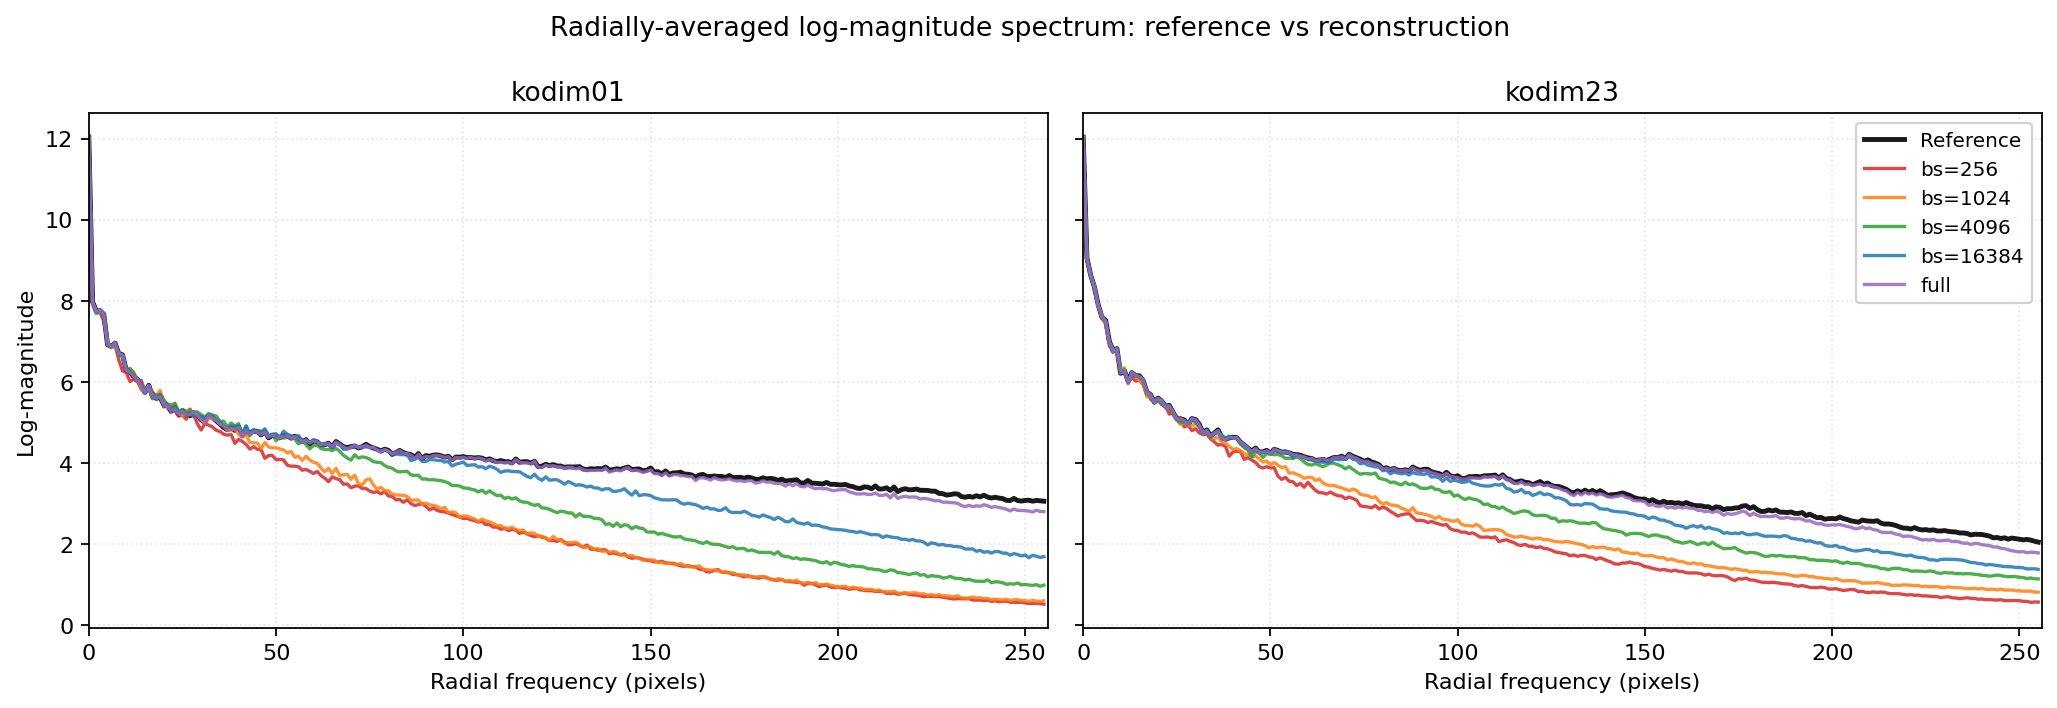
\includegraphics[width=\textwidth]{figures/radial_profiles.png}
    \caption{Radially-averaged log-magnitude spectrum for two representative
    Kodak images (\emph{kodim01}, smooth scene; \emph{kodim23}, parrot with
    fine plumage texture).  The black curve is the reference spectrum; coloured
    curves are SIREN reconstructions at different batch sizes.  All curves
    coincide at low radial frequencies; smaller batches fall below the
    reference progressively earlier as the radial frequency grows, mirroring
    the band-wise error in Table~\ref{tab:spectral_bands}.}
    \label{fig:radial_profiles}
\end{figure}

\begin{figure}[H]
    \centering
    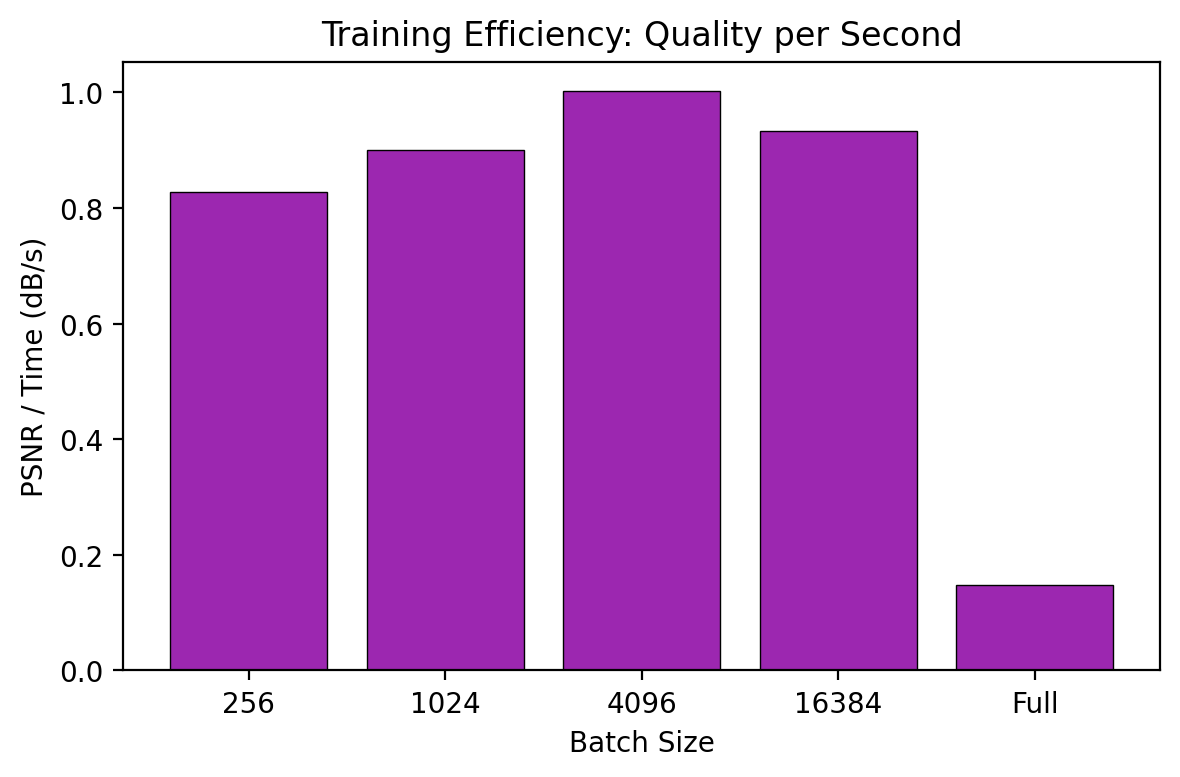
\includegraphics[width=0.85\textwidth]{figures/efficiency_vs_bs.png}
    \caption{Training efficiency: PSNR achieved per second of training time.
    Mini-batch sizes achieve more PSNR per second, but with lower quality
    ceilings.}
    \label{fig:efficiency}
\end{figure}

\begin{figure}[H]
    \centering
    \includegraphics[width=\textwidth]{figures/visual_grid_kodim01.png}
    \caption{Full reconstruction grid for kodim01. Top row: SIREN at batch
    sizes 256, 1024, 4096, 16384, full. Bottom row: COIN at the same batch
    sizes. Visual quality degrades progressively, with fine textures lost
    first.}
    \label{fig:visual_grid_full}
\end{figure}

\begin{figure}[H]
    \centering
    \includegraphics[width=\textwidth]{figures/visual_grid_kodim23.png}
    \caption{Reconstruction grid for kodim23 (a high-frequency texture image).
    The effect of batch size is even more pronounced on textured content,
    as fine patterns are among the first to degrade.}
    \label{fig:visual_grid_kodim23}
\end{figure}

\subsection{Iso-Time Visualization}

\begin{figure}[H]
    \centering
    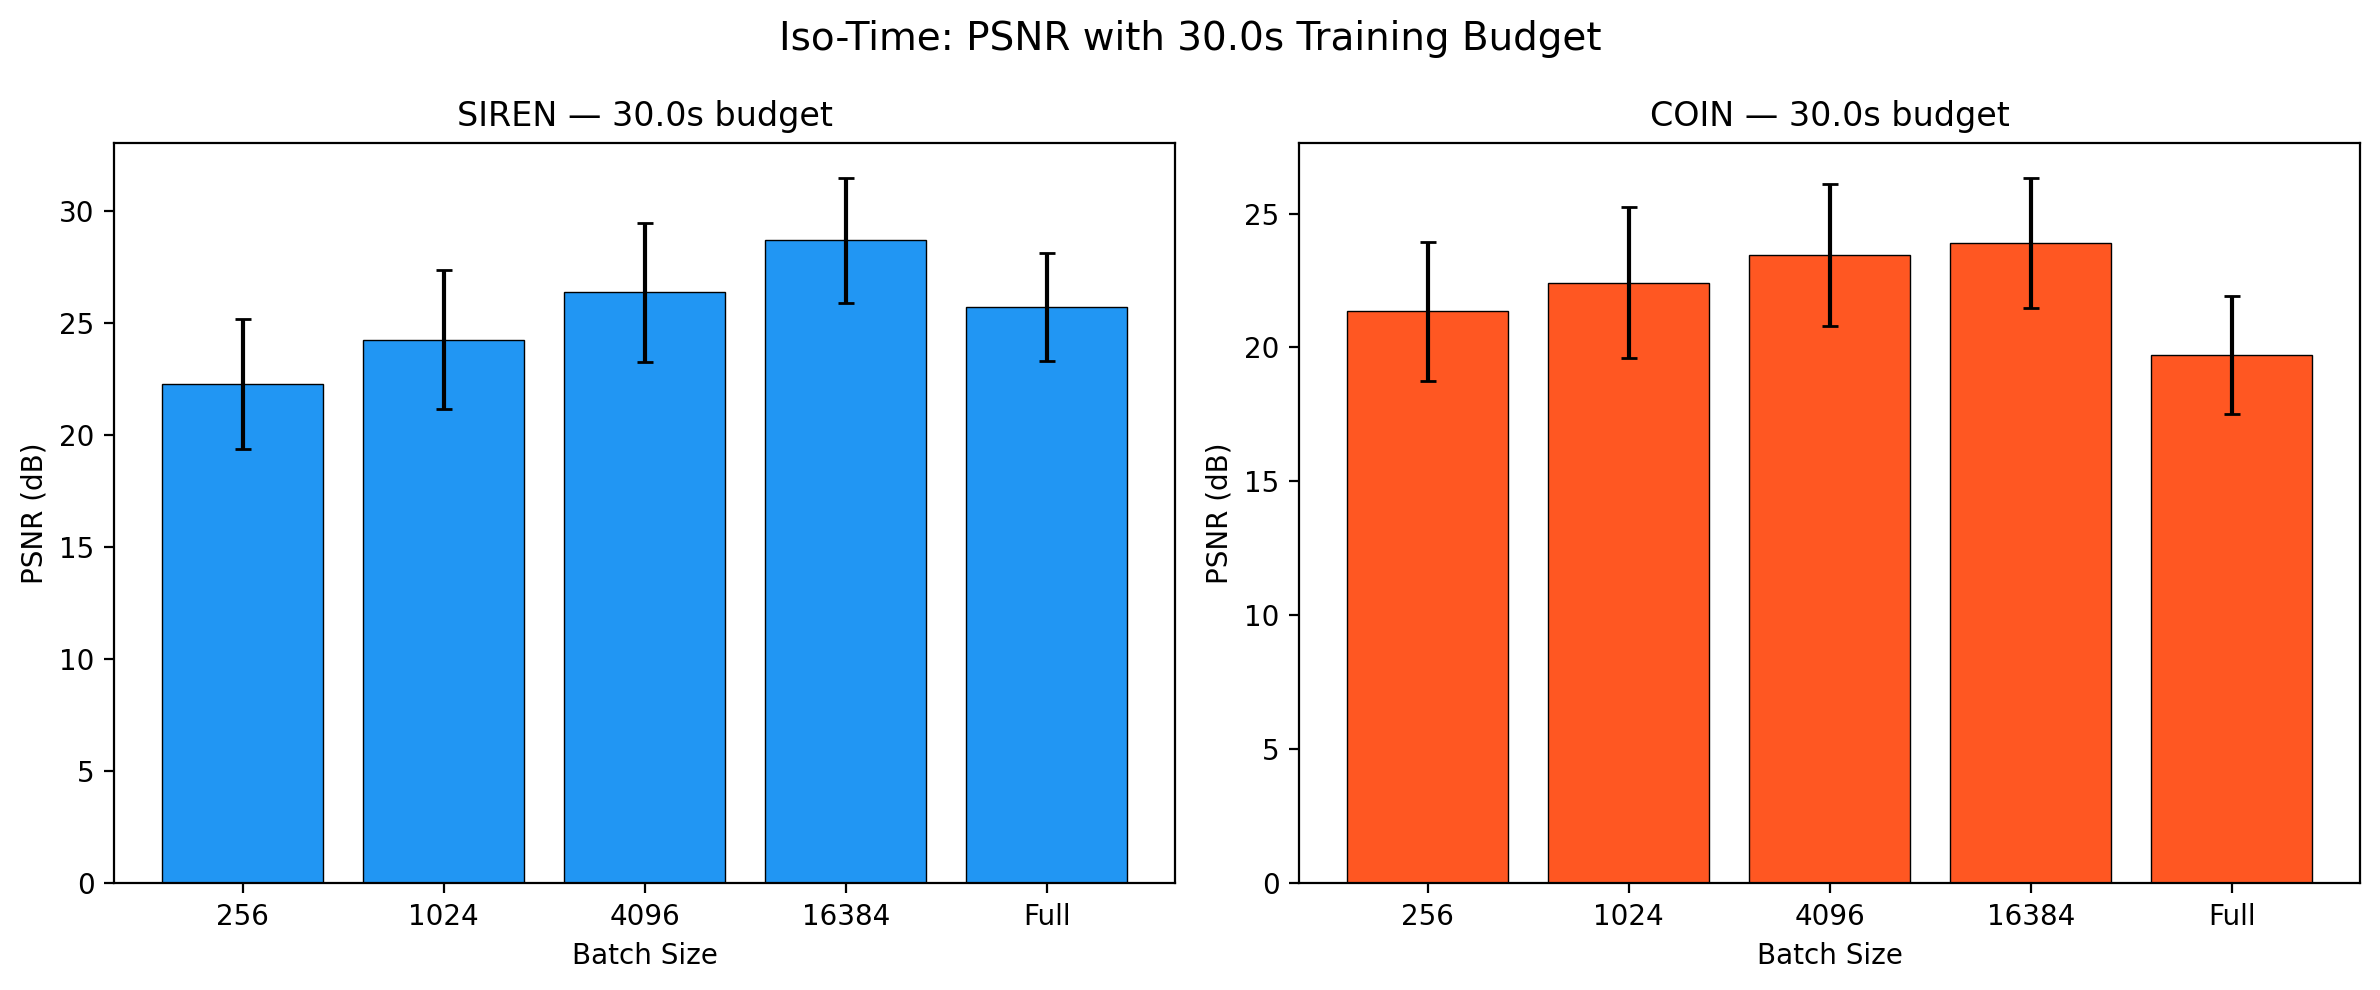
\includegraphics[width=\textwidth]{figures/iso_time_30s.png}
    \caption{Iso-time comparison at 30\,s budget. \texttt{bs=16384} is optimal
    for both architectures; full-batch completes too few steps to converge.}
    \label{fig:iso_time_30s}
\end{figure}

\begin{figure}[H]
    \centering
    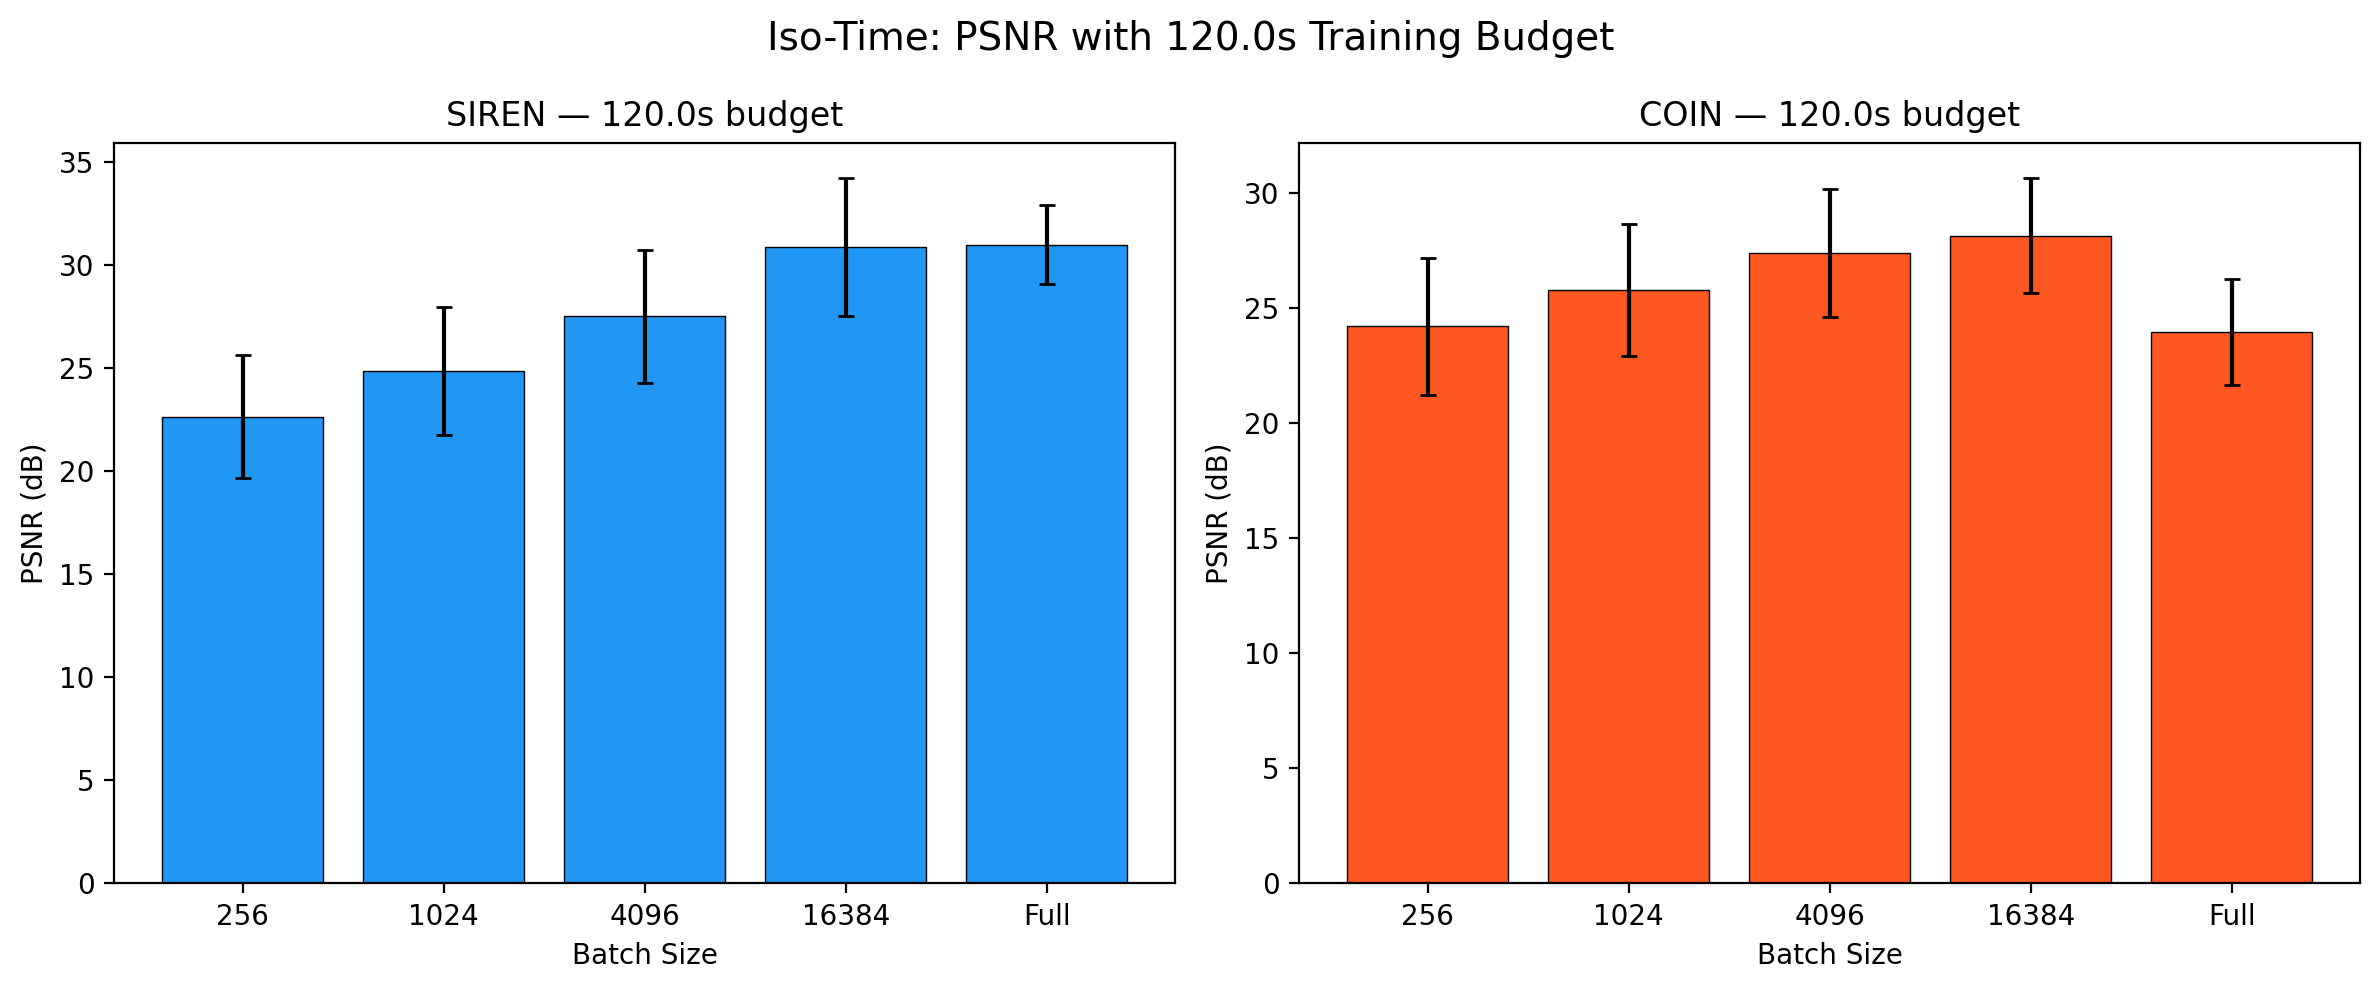
\includegraphics[width=\textwidth]{figures/iso_time_120s.png}
    \caption{Iso-time comparison at 120\,s budget. Full-batch catches up for
    SIREN but remains suboptimal for COIN.}
    \label{fig:iso_time_120s}
\end{figure}

\subsection{Adaptive Schedule Visualization}

\begin{figure}[H]
    \centering
    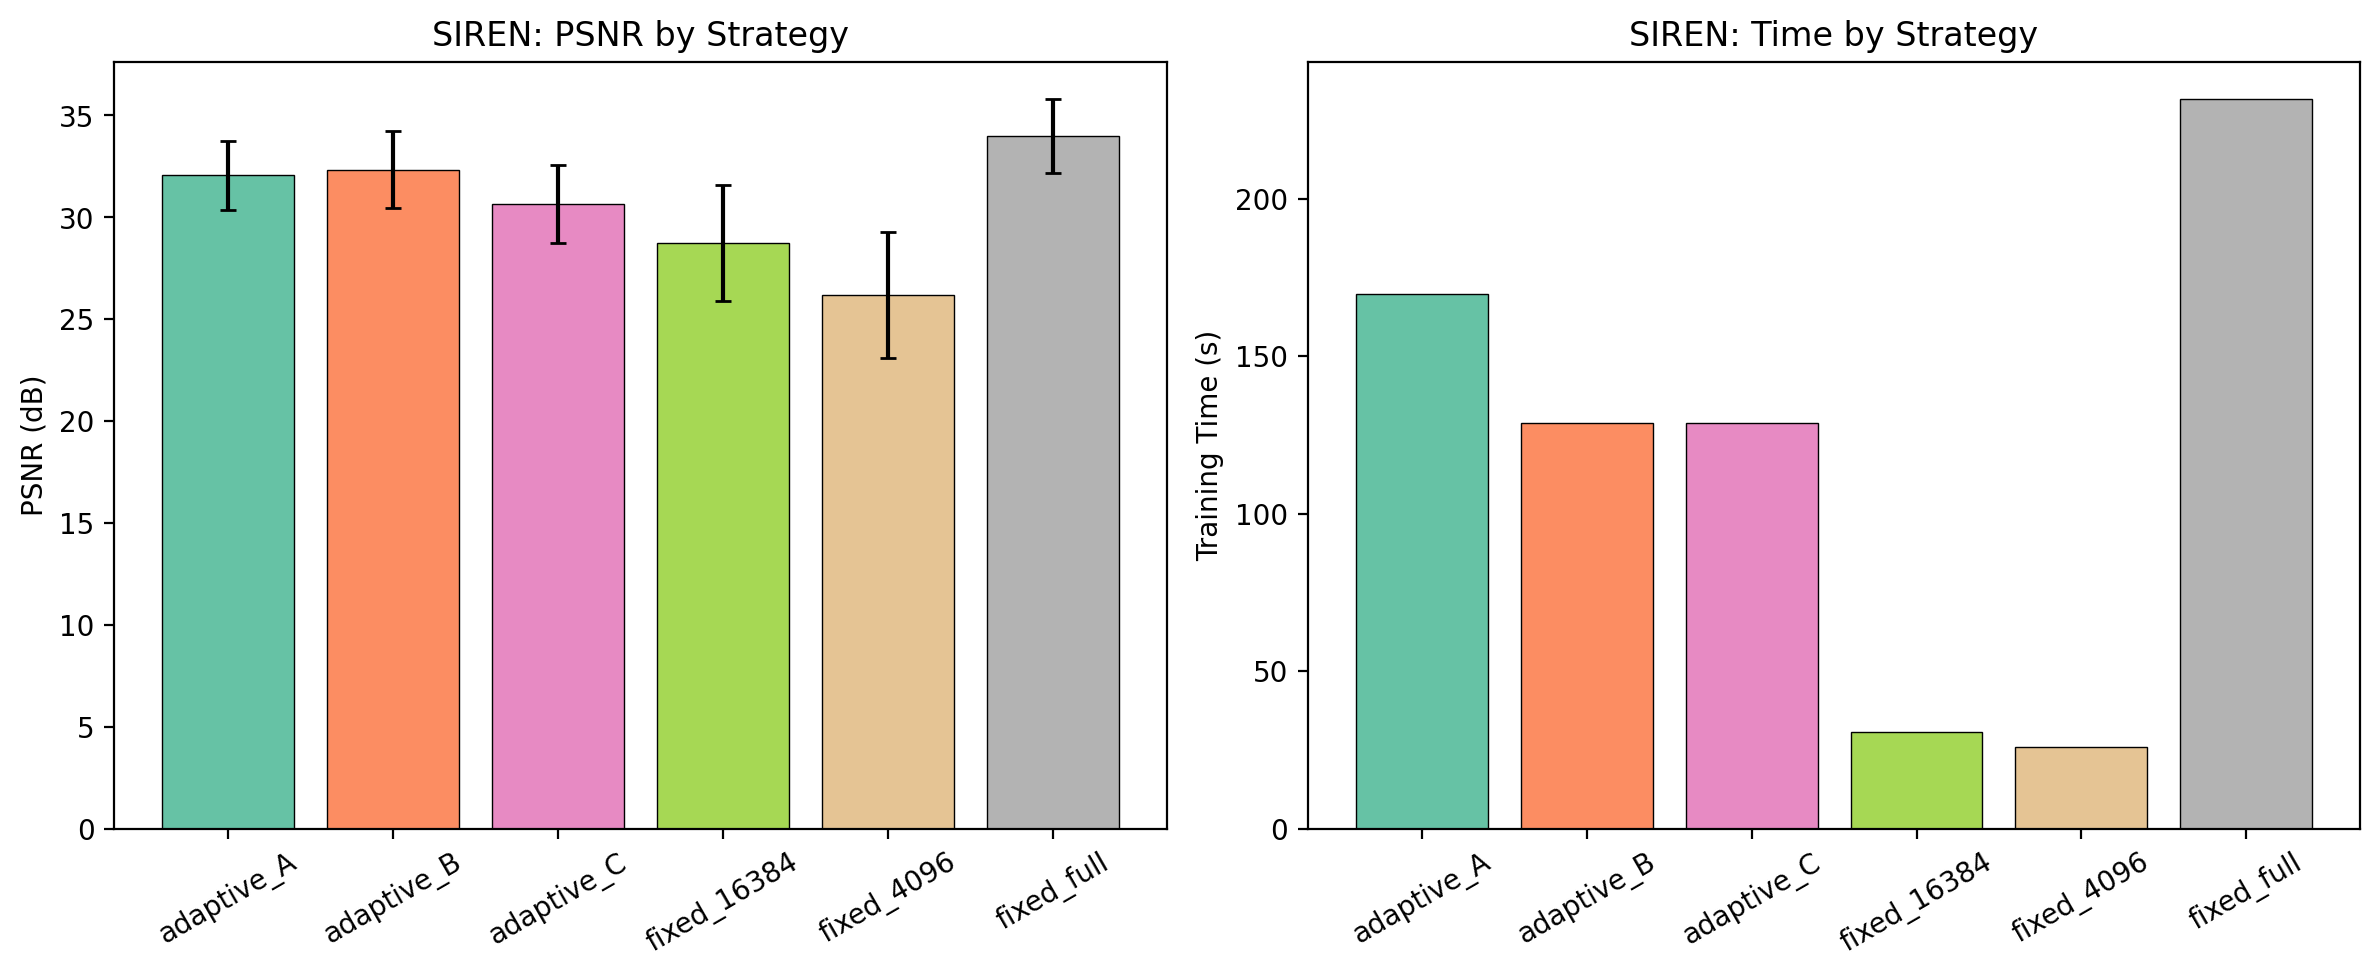
\includegraphics[width=\textwidth]{figures/adaptive_siren.png}
    \caption{Adaptive schedule performance for SIREN. Schedule B (50\% at
    bs=4096, then 50\% at full) achieves the best quality-time trade-off.}
    \label{fig:adaptive_siren}
\end{figure}

\subsection{Spectral Analysis Examples}

\begin{figure}[H]
    \centering
    \begin{subfigure}[t]{0.48\textwidth}
        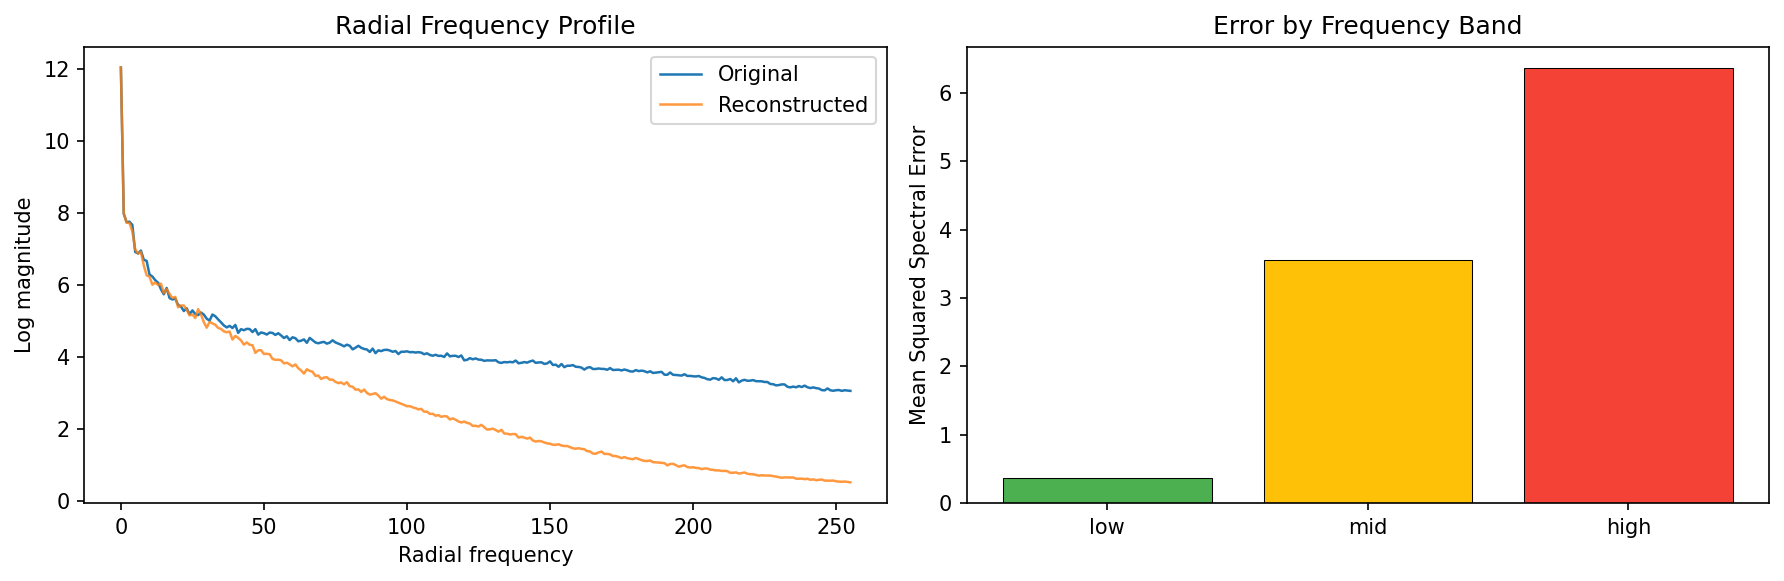
\includegraphics[width=\textwidth]{figures/spectral_kodim01_bs256.png}
        \caption{bs=256: significant high-frequency loss}
    \end{subfigure}
    \hfill
    \begin{subfigure}[t]{0.48\textwidth}
        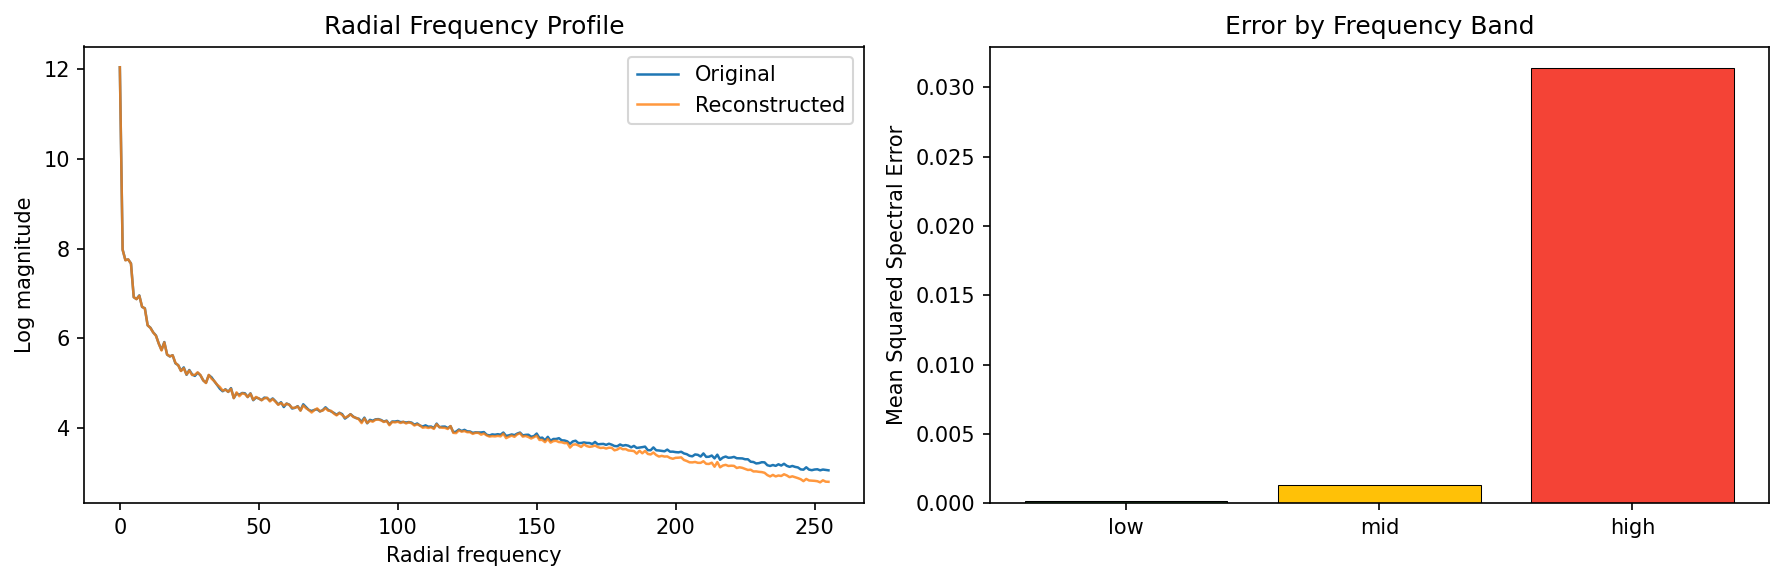
\includegraphics[width=\textwidth]{figures/spectral_kodim01_bsfull.png}
        \caption{Full-batch: faithful frequency reproduction}
    \end{subfigure}
    \caption{Spectral error maps for kodim01 at two extreme batch sizes.
    The left panel shows substantial energy loss in the high-frequency ring
    (outer region), while the right panel preserves most spectral content.}
    \label{fig:spectral_comparison}
\end{figure}

\subsection{Per-Image Summaries}

\begin{figure}[H]
    \centering
    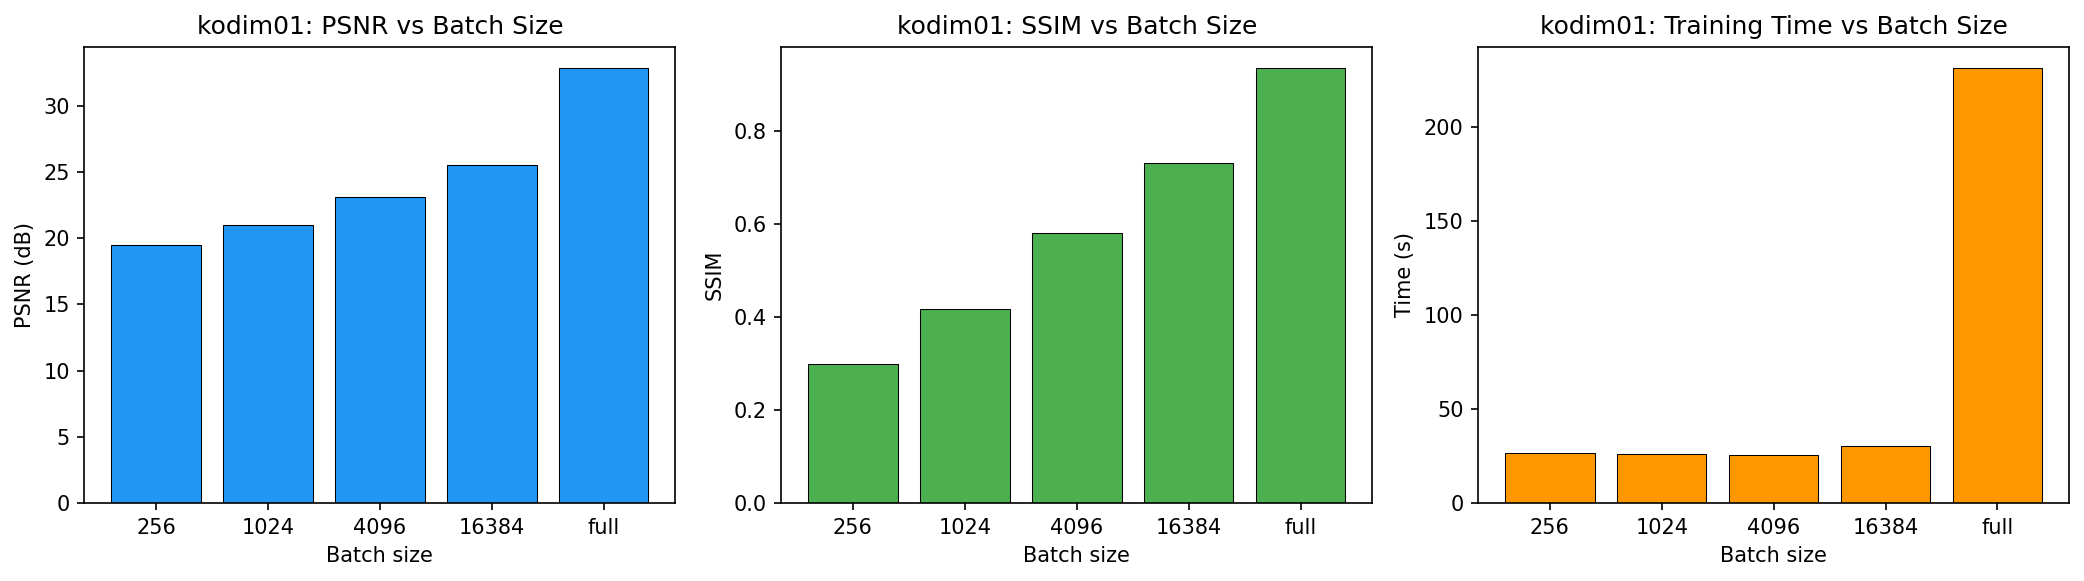
\includegraphics[width=\textwidth]{figures/summary_kodim01.png}
    \caption{Per-batch-size summary for kodim01: reconstruction quality,
    loss curve, and spectral analysis in a single view.}
    \label{fig:summary_kodim01}
\end{figure}

\begin{figure}[H]
    \centering
    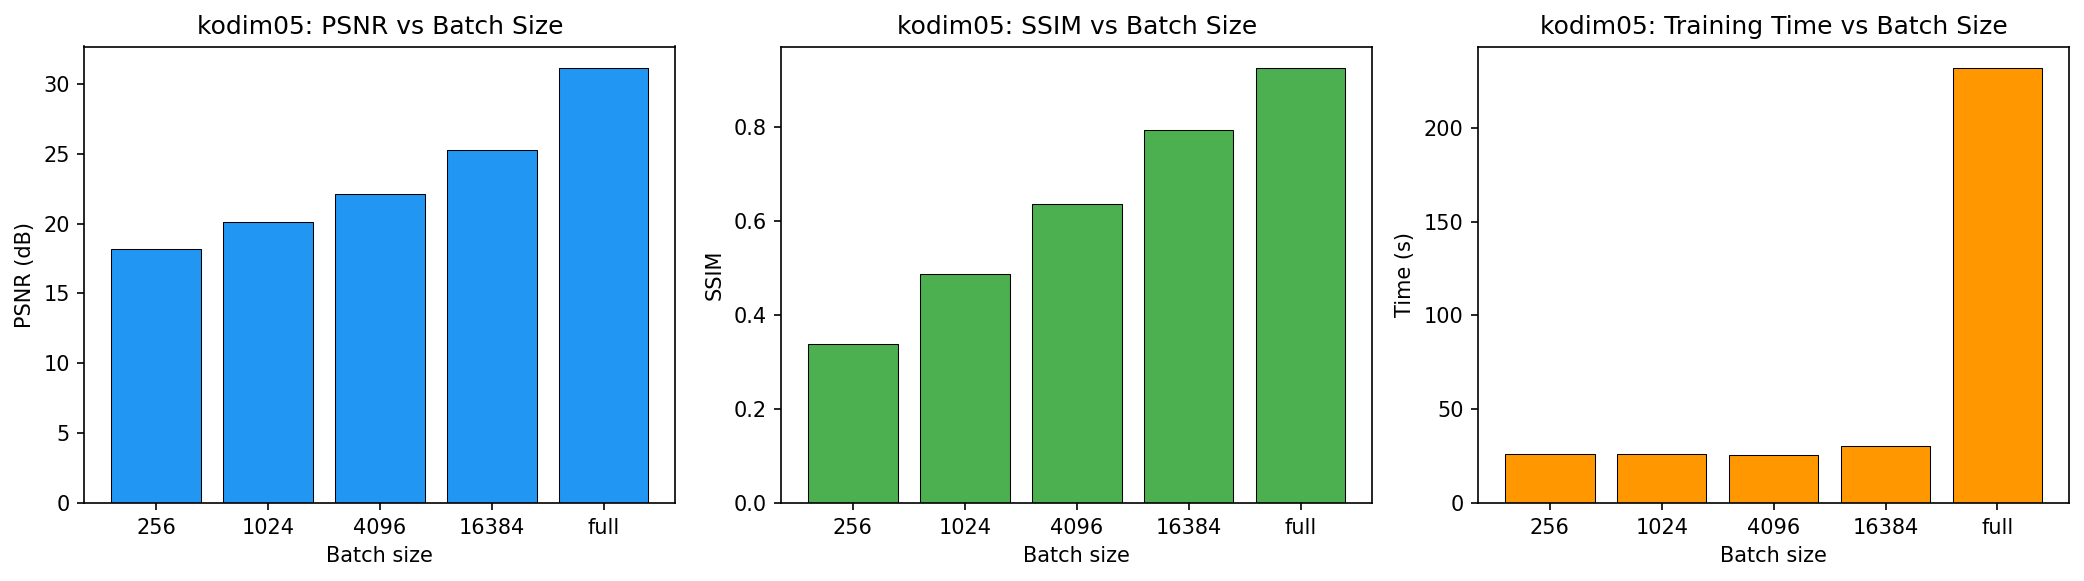
\includegraphics[width=\textwidth]{figures/summary_kodim05.png}
    \caption{Per-batch-size summary for kodim05 (low-texture landscape).
    Even for simpler images, the batch size effect is pronounced.}
    \label{fig:summary_kodim05}
\end{figure}

\begin{figure}[H]
    \centering
    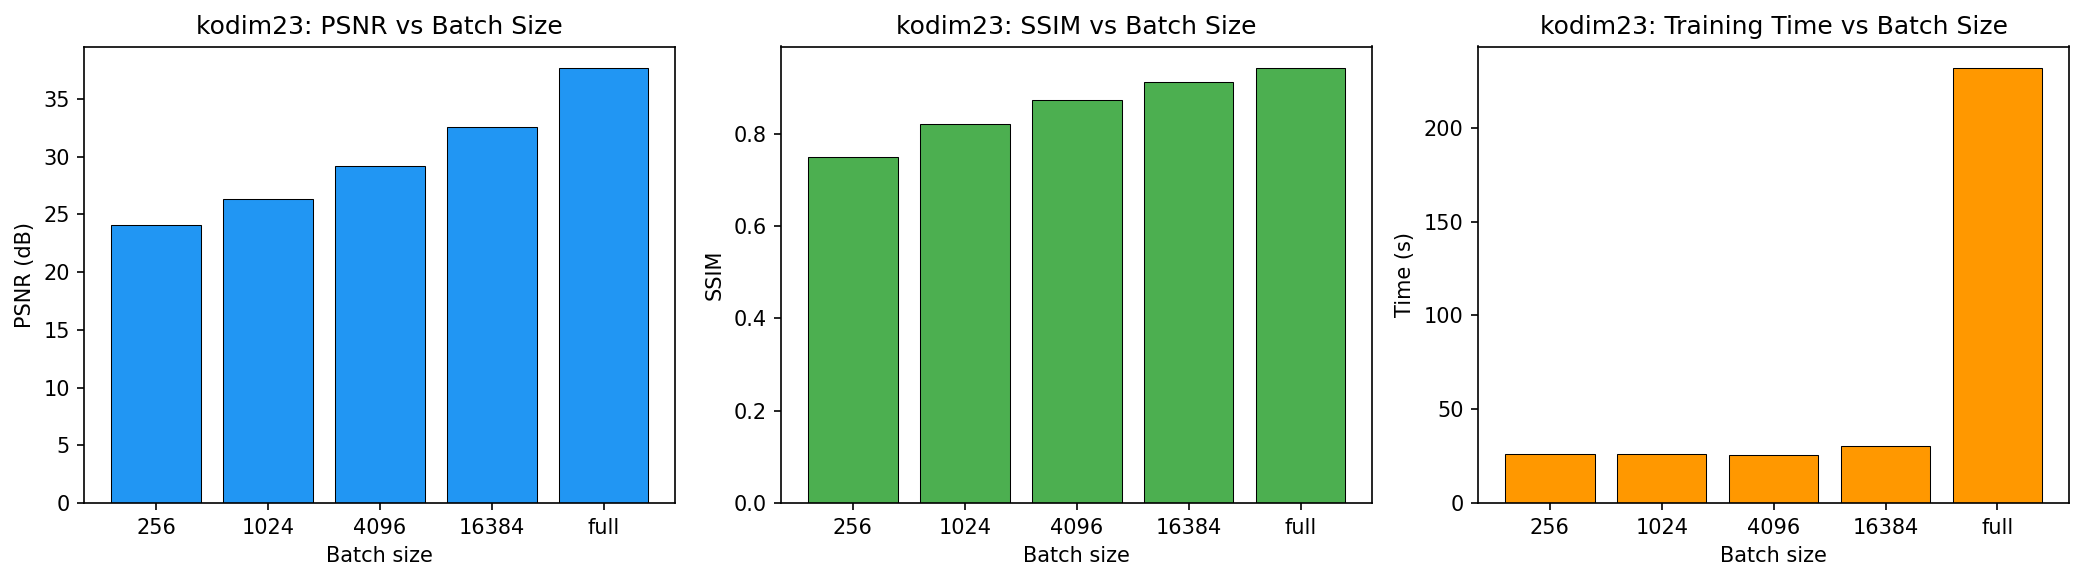
\includegraphics[width=\textwidth]{figures/summary_kodim23.png}
    \caption{Per-batch-size summary for kodim23 (high-frequency building
    facade). This image shows one of the largest batch size sensitivities
    in the dataset.}
    \label{fig:summary_kodim23}
\end{figure}

\section{Experiment Summary}
\label{app:experiment_summary}

\begin{table}[H]
\centering
\caption{Complete list of all experiments conducted in this study.}
\label{tab:all_experiments}
\begin{tabular}{clcc}
\toprule
\# & Experiment & Training Runs & GPU Time \\
\midrule
1  & SIREN batch-size sweep & 120 & $\sim$2.5\,h \\
2  & COIN batch-size sweep & 120 & $\sim$2.5\,h \\
3  & Iso-time comparison & 720 & $\sim$5\,h \\
4  & Adaptive scheduling & 216 & $\sim$2\,h \\
5  & Gradient variance & 150 meas. & $\sim$1\,h \\
6  & LR scaling & 96 & $\sim$1.5\,h \\
7  & Per-image difficulty & 24 & $<$1\,min \\
8  & JPEG comparison & 312 & $<$1\,min \\
9  & Multi-seed validation & 90 & $\sim$1.5\,h \\
10 & VRAM profiling & 10 & $\sim$5\,min \\
11 & Model-size ablation & 120 & $\sim$2\,h \\
\midrule
   & \textbf{Total} & $\sim$\textbf{1{,}600} & $\sim$\textbf{20\,h} \\
\bottomrule
\end{tabular}
\end{table}


\end{document}
